\documentclass[11pt,final]{tutdrthesis}
\usepackage{graphicx}
%\usepackage[dvips]{graphicx}
\usepackage{enumerate}
\usepackage{enumitem}
\usepackage[USenglish]{babel}
\usepackage{layout}
\usepackage{cite}
\usepackage{rotating}
\usepackage{amsmath}
\usepackage{multirow}
\usepackage{textcomp}
\usepackage{array, ragged2e}

% Load the package
\usepackage[acronym,nomain,nonumberlist,nopostdot,nogroupskip]{glossaries}

\usepackage{mathrsfs}

\usepackage{chngcntr}
\counterwithin{figure}{chapter}
\counterwithin{table}{chapter}

\usepackage{enumerate}
\usepackage{enumitem}
\newenvironment{packed_enumerate}{
\begin{enumerate}
  \setlength{\partopsep}{1pt}
  \setlength{\itemsep}{3pt}
  \setlength{\parskip}{1pt}
  \setlength{\parsep}{1pt}
}{\end{enumerate}}

\newlist{bold_description}{description}{1}
\setlist[bold_description]{labelindent=8mm,itemindent=2mm,leftmargin=15mm,style=sameline, font=\textbf,parsep=0pt,itemsep=0pt}

\newcommand{\longpage}{\enlargethispage*{100cm} \pagebreak}
\newcommand{\nohyphens}{\hyphenpenalty=10000\exhyphenpenalty=10000\relax}
\newcommand{\ci}[1]{\cite{#1}}

\newcommand{\mymod}{\mathop{\rm mod^*}}
\newcommand{\sgn}{\mathop{\rm sgn}}
%\newcommand{\argmax}{\mathop{\rm arg\,max}}
\newcommand{\argmin}{\mathop{\rm arg\,min}}
\newcommand{\hw}{hardware }
\newcommand{\sw}{software }
%\newcommand{\cd} {Cholesky decomposition }

\newcommand{\subsubsubsection}[1]{\paragraph{#1:}}
\newcommand{\bc}[1]{\texttt{\textbf{#1}}}
\newcommand{\lc}[1]{\texttt{#1}}

%\setglossarystyle{long}

\setlength{\glsdescwidth}{0.7\linewidth}%
%\setlength\extrarowheight{12pt}%

\newcolumntype{R}{>{\raggedright\arraybackslash}p{\glsdescwidth}}

\newglossarystyle{clong}{%
 \renewenvironment{theglossary}%
     {\begin{longtable}[l]{p{.2\linewidth}R	p{\glsdescwidth}}}%    
     {\end{longtable}}%
  %\renewcommand*{\glsclearpage}{\clearpage}   
  \renewcommand*{\glossaryheader}{}%
  \renewcommand*{\glsgroupheading}[1]{}%
  \renewcommand*{\glossaryentryfield}[5]{%
    \glstarget{##1}{##2} & ##3\glspostdescription\space\\ ##5}%
  \renewcommand*{\glossarysubentryfield}[6]{%
     & \glstarget{##2}{\strut}##4\glspostdescription\space ##6\\}%
  %\renewcommand*{\glsgroupskip}{ & \\}%
}

%%%%%%%%%%%%%%%%%%%%%%%%%%%%%%%%%%%%%%%%%%%%%%%%%%%%%%%%%%%%%%%%%%%%%%%%%%%%%%%
%
% Custom math symbols
%
%%%%%%%%%%%%%%%%%%%%%%%%%%%%%%%%%%%%%%%%%%%%%%%%%%%%%%%%%%%%%%%%%%%%%%%%%%%%%%%

\DeclareMathOperator*{\argmax}{arg\,max}
\DeclareMathAlphabet{\mathpzc}{OT1}{pzc}{m}{it}

%\hyphenation{ACS}
%\hyphenation{ACSU}
%\hyphenation{ACSUs}
\hyphenation{FFT}
\hyphenation{MAC}
\hyphenation{GPP}
\hyphenation{DPS}
\hyphenation{ASIC}
\hyphenation{ASP}

% Generate the glossary
\makeglossaries

%%%%%%%%%%%%%%%%%%%%%%%%%%%%%%%%%%%%%%%%%%%%%%%%%%%%%%%%%%%%%%%%%%%%%%%%%%%%%%
%                                                                            %
% CONTENT BEGINS                                                             % 
%                                                                            %
%%%%%%%%%%%%%%%%%%%%%%%%%%%%%%%%%%%%%%%%%%%%%%%%%%%%%%%%%%%%%%%%%%%%%%%%%%%%%%
\begin{document}

%\thispagestyle{empty}
%
\includegraphics[width=8cm]{Text/tut-logo}
%\degree{Doctoral thesis}
\author{Robert E. Guinness}
\title{Context Awareness for Navigation Applications}
\subtitle{Doctoral thesis}
\maketitle
% 
% \vspace*{-.5cm}\noindent
% 
% % If thesis is in English, use the file "tut-logo"
% % instead of "tty-logo" in the following:
% 
% 
% 
% \vspace{2.8cm}
% 
% \noindent{\normalsize \textsf{Robert E. Guinness}}\\ \\
% {\bf\large \textsf{Context Awareness for Navigation Applications}}\\ \\
% \textsf{Doctoral thesis}\\ \\

%\vspace{8.7cm} % jos kaksi otsikkoriviä vaihda -> 6.7cm

%\begin{flushright}
%
%\begin{minipage}[c]{6.8cm}
%\begin{spacing}{1.0}
%\textsf{Tarkastaja: Tarkastaja 1}\\
%\textsf{Tarkastaja ja aihe hyväksytty}\\
%\textsf{xxxxxxx tiedekuntaneuvoston}\\
%\textsf{kokouksessa xx.xx.xxxx}\\
%\end{spacing}
%\end{minipage}
%\end{flushright}

\frontmatter
\setcounter{secnumdepth}{-1}

\chapter{Abstract}
TBD
\chapter{Preface}
The research work presented in this thesis was carried out between November 2011 and May 2014. I have chosen to complete a ``compendium-style'' dissertation, in part because I have already had the pleasure of preparing a monograph when co-authoring a book with Prof. Ruizhi Chen, published in July 2014. I have no great desire to repeat such an experience yet. As many who have published such monographs can attest, it takes a lot out of you!

Due to other responsibilities, as well as a bad case of the ``it's-not-good-enough-yet'' syndrome, it took me more than one year to finalize and publish some of the results of my doctoral research in article format. With the aid of gentle nudging from my colleagues and superiors, I prepared the summary content for this compendium mostly between January and July 2015.

There are two particular experiences I'd like to share that also motivated me for completing this dissertation. The first is when I was asked to be a reviewer for an article submitted to one highly-esteemed journal. When I realized that my work, in my own opinion, was superior to that which I was reviewing, I felt suddenly cured of the above-mentioned syndrome. This is one of the side benefits of peer review. The second was when I was participating in an interview of a beloved colleague (he got the job!). We asked him if he could describe one achievement of which he was most proud. Instead of pointing to one particular academic achievement, such as a highly-cited paper, he pointed out another kind of achievement: the fact that he can look back at his publications and realize that some of the early ones were poor but that there has been a steady improvement in the quality over the years. Since hearing that, this is what I aim for: Not to publish the perfect gem some day but to continually put out my work-in-progress for others to see and hopefully benefit from.

Thank yous....

% The thesis text is written into file \texttt{d\_tyo.tex}, whereas
% \texttt{tutthesis.cls} contains the formatting instructions. Both
% files include lots of comments (start with \%) that should help in
% using LaTeX. TUT specific formatting is done by additional settings on
% top of the original \texttt{report.cls} class file. This example needs
% few additional files: TUT logo, example figure, example code, as well
% as example bibliography and its formatting (\texttt{.bst}) An example
% makefile is provided for those preferring command line. You are
% encouraged to comment your work and to keep the length of lines
% moderate, e.g. <80 characters. In Emacs, you can use \texttt{Alt-Q} to
% break long lines in a paragraph and \texttt{Tab} to indent commands
% (e.g. inside figure and table environments). Moreover, tex files are
% well suited for versioning systems, such as Subversion or Git.  
% % \url{http://www.ctan.org/tex-archive/info/lshort/english/lshort.pdf}
% 
% 
% Acknowledgements to those who contributed to the thesis are generally
% presented in the preface. It is not appropriate to criticize anyone in
% the preface, even though the preface will not affect your grade. The
% preface must fit on one page. Add the date, after which you have not
% made any revisions to the text, at the end of the preface.

~ 
% Tilde ~ makes an non-breakable spce in LaTeX. Here it is used to get
% two consecutive paragraph breaks

Kirkkonummi, X.Y.2015

~


Robert E. Guinness
\chapter{Table of Contents}
\tableofcontents
%\chapter{List of Publications}
%%This thesis contains a compilation of five previously published papers, referred to as [P\#] throughout the text. The following publications are included:

\begin{itemize}
\item [P1]
\item [P2]
\item [P3]
\item [P4]
\item [P5]
\end{itemize}

\chapter{List of Figures}
\listoffigures
\chapter{List of Tables}
\listoftables

\chapter{Abbreviations}

\newacronym{ai}{AI}{Artificial Intelligence}
\newacronym{mems}{MEMS}{microelectromechanical systems}
\newacronym{plc}{PLC}{Propositional Logic of Context}
\newacronym{locomo}{LoCoMo}{Location-Motion-Context}
\newacronym{lsa}{LSA}{latent semantic analysis}
\newacronym{pca}{PCA}{principal component analysis}
\newacronym{bc}{BC}{Before Christ}
\newacronym{fiveWs}{Five Ws}{Who, What, Where, When, and Why}
\newacronym{wgs84}{WGS84}{World Geodetic System 1984}
\newacronym{n}{N}{North}
\newacronym{e}{E}{East}
\newacronym{os}{OS}{Operating System}
\newacronym{gps}{GPS}{Global Positioning System}
\newacronym{rgb}{RGB}{Red, Green, and Blue}
\newacronym{sql}{SQL}{Structured Query Language}
\newacronym{ibm}{IBM}{International Business Machines Corporation}
\newacronym{jmc}{jmc}{John McCarthy}
\newacronym{fide}{FIDE}{Federation Internationale des Echecs}
\newacronym{optics}{OPTICS}{ordering points to identify the clustering structure}
\newacronym{em}{EM}{expectation-maximization}
\newacronym{gmm}{GMM}{Guassian mixture model}
\newacronym{mle}{MLE}{maximum likelihood estimate}
\newacronym{inosense}{INOSENSE}{Indoor Outdoor Seamless Navigation for Sensing Human Behavior}
\newacronym{aess}{AESS}{Aerospace and Electronics Systems Society}
\newacronym{ion}{ION}{Institute of Navigation}
\newacronym{ieee}{IEEE}{Institute of Electrical and Electronics Engineers}
\newacronym{arcsat}{ARCSAT}{Arctic Real-Time Satellite Services for the Public and Commercial End-Use}
\newacronym{esabalt}{ESABALT}{Enhanced Situational Awareness to Improve Maritime Safety in the Baltic}
\newacronym{svm}{SVM}{Support Vector Machines}
\newacronym{jufo}{JuFo}{Julkaisufoorumi (Finnish for ``Publications forum'')}
\newacronym{plans}{PLANS}{Position Location and Navigation Symposium}
\newacronym{wlan}{WLAN}{wireless local area network}
\newacronym{fgi}{FGI}{Finnish Geospatial Research Institute (prior to 2015: Finnish Geodetic Institute)}
\newacronym{lms}{LMS}{local models semantics}
\newacronym{cil}{CIL}{Contextual Intensional Logic}
\newacronym{uci}{UCI}{University of California, Irvine} 

%\begin{tabular}{l@{\hspace{0.8cm}}l}
%\setlength{\tabcolsep}{50mm}
AVUPT & Absolute Visual attitude Update\\ [2.0ex]
BLUE & Best Linear Unbiased Estimate\\[2.0ex]
C/A & Coarse/Acquisition\\[2.0ex]
CCD & Charge Coupled Device\\[2.0ex]
CMOS & Complementary Metal Oxide Semiconductor\\[2.0ex]
COMPASS/Beidou & Chinese Satellite Navigation System\\[2.0ex]
DCM & Direction Cosine Matrix\\[2.0ex]
DOP & Dilution Of Precision\\[2.0ex]
E & East\\[2.0ex]
ECEF & Earth Centered Earth Fixed\\[2.0ex]
EKF & Extended Kalman Filter\\[2.0ex]
ENU & East-North-Up\\[2.0ex]
EXIF & Exchangeable Image File\\[2.0ex]
Galileo & European Satellite Navigation System\\[2.0ex]
GDOP & Geometric Dilution Of Precision\\[2.0ex]
GLONASS & The Russian Positioning System, Global'naya \\[0.5ex]
& Navigatsionnaya Sputknikkovaya Sistema\\[2.0ex]
GNSS & Global Navigation Satellite System\\[2.0ex]
\end{tabular}
\newpage
\begin{tabular}{l@{\hspace{2cm}}l}
GPS & Global Positioning System\\[2.0ex]
HD & High-definition\\[2.0ex]
HSGPS & High Sensitivity GPS\\[2.0ex]
IEEE & The Institute of Electrical and Electronics Engineers\\[2.0ex]
ION & Institute of Navigation\\[2.0ex]
IMU & Inertial Measurement Unit\\[2.0ex]
INS & Inertial Navigation System\\[2.0ex]
KF & Kalman filter\\[2.0ex]
LCI & Low-coherence Interferometry\\[2.0ex]
LDOP & Line Dilution Of Precision\\[2.0ex]
LOS & Line Of Sight\\[2.0ex]
Max & Maximum\\[2.0ex]
MEMS & Micro-Electro-Mechanical\\[2.0ex]
Min & Minimum\\[2.0ex]
MSP & Multi Sensor Positioning\\[2.0ex]
N & North\\[2.0ex]
PGCP & Pseudo Ground Control Points\\[2.0ex]
PDOP & Position Dilution Of Precision\\[2.0ex]
PPP & Precise Point Positioning\\[2.0ex]
RANSAC & RANdom SAmple Consensus\\[2.0ex]
\end{tabular}
\newpage
\begin{tabular}{l@{\hspace{2cm}}l}
\setlength{\tabcolsep}{50mm}
RF & Radio Frequency\\[2.0ex]
RFID & Radio Frequency Identification\\[2.0ex]
rms & root mean square\\[2.0ex]
RSSI & Received Signal Strength Indication\\[2.0ex]
SHT & Standard Hough Tranform\\[2.0ex]
SIFT & Scale Invariant Feature Transform\\[2.0ex]
SLAM & Simultaneous Localization And Mapping\\[2.0ex]
SPAN & Synchronized Position Attitude Navigation\\[2.0ex]
SVD & Singular Value Decomposition\\[2.0ex]
std & standard deviation\\[2.0ex]
ToA & Time of Arrival\\[2.0ex]
TVUPT & Temporal Visual Attitude Update\\[2.0ex]
U & Up\\[2.0ex]
UAV & Unmanned Aerial Vehicle\\[2.0ex]
UKF & Unscented Kalman filter\\[2.0ex]
UTC & Coordinated Universal Time\\[2.0ex]
UERE & User Equivalent Range Error\\[2.0ex]
UWB & Ultra-Wideband\\[2.0ex]
VA & Vision-aided\\[2.0ex]
WiFi & Wireless network, a registered trademark of the Wi-Fi Alliance\\[2.0ex]
WLAN & Wireless Local Area Network\\[2.0ex]
\end{tabular}


%Print the glossary
\begingroup
%\let\newpage\relax
\setlength\extrarowheight{12pt}
%\let\glscleardoublepage\relax
%\let\glsclearpage\relax
\let\clearpage\relax 
%\let\glossarypreamble\relax
\vspace{-8.5em}
\printglossary[type=\acronymtype,style=clong]
\endgroup

\chapter{Symbols}

%To be replaced with my own list (This one from Laura)\\
\begin{tabular}{l@{\hspace{3cm}}l}
$\alpha_i$ & Angle between a line $i$ in an image and the image x-axis\\[2.0ex]
$\beta$ & roll\\[2.0ex]
$\Delta t$ & Time interval\\[2.0ex]
$\Delta \mathbf x$ & Vector offset of the user's true position and time bias\\[0.5ex]
{} & from the values at the linearization point\\[2.0ex]
$\delta \mathbf x_k$ & Perturbation of the state\\[2.0ex]
$\epsilon^-$ & Error of \textit{a priori} state estimate or perturbation of the\\[0.5ex]
{} & Euler angles\\[2.0ex]
$\epsilon$ & Error of \textit{a posteriori} state estimate or noise\\[0.5ex]
{} & in GPS measurements \\[0.5ex]
{} & or vector of errors in GNSS measurements\\[2.0ex]
$\eta_g$ & Noise in gyroscope or carrier phase measurement\\[2.0ex]
$\lambda$ & Carrier wavelength or longitude\\[2.0ex]
$\mu$ & Mean\\[2.0ex]
$\nabla$ & Image gradient\\[2.0ex]
$\omega$ & Earth turn rate\\[2.0ex]
$\omega_{ib}^b$ & Body (b) turn rate with respect to the inertial (i) frame\\[0.5ex]
{} & angular velocity measurement\\[2.0ex]
$\tilde\omega_{ib}^b$ & Gyroscope angular velocity measurement\\[2.0ex]
\end{tabular}

\newpage
\begin{tabular}{l@{\hspace{3cm}}l}
$\mathbf\Omega$ & Skew symmetrical matrix of the angular velocity vector\\[2.0ex]
$\phi$ & pitch or latitude\\[2.0ex]
$\mathbf \Phi$ & State transition matrix\\[2.0ex]
$\rho$ & Pseudorange or the radius of a line in an image in \\[0.5ex]
{} & Hough Transform \\[2.0ex]
$\hat\rho$ & Estimated pseudorange computed from the estimated\\[0.5ex]
{} &  user position\\[2.0ex]
$\sigma$ & Standard deviation\\[2.0ex]
$\sigma^2$ & Variance\\[2.0ex]
$\sigma^2_C(t_A)$ & Allan variance\\[2.0ex]
$\theta$ & Heading, (azimuth) \\ [2.0ex]
$\varphi$ & Carrier phase\\[2.0ex]
$b$ & body frame\\[2.0ex]
$c$ & Speed of light\\[2.0ex]
$\mathbf C$ & Direction cosine matrix or Convolution\\[2.0ex]
$\mathbf d$ & direction of a line in an image\\[2.0ex]
$d_{iono}$ & Ionospheric delay\\[2.0ex]
$d_{tropo}$ & Tropospheric delay\\[2.0ex]
$d\rho$ & Ephemeris error\\[2.0ex]
$dt$ & Satellite clock error\\[2.0ex]
$D_i$ & Distance between the starting point of line $i$\\[0.5ex]
{} & and the vanishing point\\[2.0ex]
$\mathbf E$ & Essential matrix\\[2.0ex]
$f$ & Focal legth\\[2.0ex]
$\mathbf f$ & Specific force\\[2.0ex]
\end{tabular}
\newpage
\begin{tabular}{l@{\hspace{3cm}}l}
$\mathbf F$ & Fundamental matrix\\[0.5ex]
$\mathbf g$ & Mass gravitation\\[2.0ex]
$\mathbf G$ & User-satellite geometry matrix or Convolution kernel\\[0.5ex]
{} &  or g-sensitivity coefficient matrix\\[2.0ex]
$h$ & Height\\[2.0ex]
$H$ & Height of an image in pixels\\[2.0ex]
$\mathbf H$ & Design matrix or image homography\\[2.0ex]
$i$ & inertial frame\\[2.0ex]
$\mathbf I$ & Image matrix\\[2.0ex]
$k$ & Distortion value\\[2.0ex]
$\mathbf K$ & Kalman gain or camera calibration matrix\\[2.0ex]
L1 & GPS signal carrier frequency at 1575.42 MHz\\[2.0ex]
$\mathbf M$ & Image gradient magnitude matrix\\[2.0ex]
$N$ & Gaussian probability distribution or integer number\\[0.5ex]
{} & of carrier waves\\[2.0ex]
$N^e$ & Inertia tensor\\[2.0ex]
$\mathbf O$ & Image gradient orientation matrix\\[2.0ex]
$p$ & pressure\\[2.0ex]
$\mathbf P$ & State error covariance or camera matrix\\[2.0ex]
$\tilde q$ & Spectral density value\\[2.0ex]
$\mathbf Q$ & Process noise covariance\\[2.0ex]
$r$ & Geometric range\\[2.0ex]
$r_d$ & Radial distance of the normalized distorted image point\\[2.0ex]
$\mathbf r$ & User position vector or Least-squares residual vector\\[2.0ex]
\end{tabular}
\newpage
\begin{tabular}{l@{\hspace{3cm}}l}
\setlength{\tabcolsep}{50mm}
$\mathbf R$ & Measurement noise covariance or camera rotation\\[0.5ex]
{} &  matrix\\[2.0ex]
$R_g$ & Universal gas constant\\[2.0ex]
$\mathbf{R}_{WLAN}$ & RSSI observation vector\\[2.0ex]
$s$ & Ambiguous scale in translation observed from\\[0.5ex]
{} & consecutive images\\[2.0ex]
$\mathbf s$ & Satellite coordinate vector\\[2.0ex]
$S$ & User speed\\[2.0ex]
$\mathbf S$ & Scale factor and non-orthogonality matrix\\[2.0ex]
$t$ & time\\[2.0ex]
$t_u$ & Receiver clock error\\[2.0ex]
$\mathbf t$ & User translation vector\\[2.0ex]
$\mathbf T^i$ &Satellite i's position vector \\[2.0ex]
$\mathbf T_{rcvr}$ &Receiver position vector \\[2.0ex]
$T_0$ & Temperature at the sea level\\[2.0ex]
$T_L$ & Temperature lapse rate\\[2.0ex]
$u$ & Principal point's x-coordinate\\[2.0ex]
$\mathbf u$ & User coordinate vector\\[0.5ex]
{} & or the unit vector from user to satellite\\[2.0ex]
$u_{GC}$ & Satellite and user geometry change\\[2.0ex]
$v$ & Principal point's y-coordinate\\[2.0ex]
$\mathbf v$ & Kalman filter's innovation vector\\[0.5ex]
{} &  or user velocity vector or a vanishing point matrix\\[2.0ex]
$v_k$ & Process noise\\[2.0ex]
\end{tabular}
\newpage
\begin{tabular}{l@{\hspace{3cm}}l}
$vfov$ & Vertical field-of-view of a camera\\[2.0ex]
$\mathbf v_x$ & Vanishing point in x-axis direction\\[0.5ex]
{} & in homogenous coordinates\\[2.0ex]
$\mathbf v_y$ & Vanishing point in y-axis direction\\[0.5ex]
{} & in homogenous coordinates\\[2.0ex]
$\mathbf v_z$ & Vanishing point in z-axis direction\\[0.5ex]
{} & in homogenous coordinates\\[2.0ex]
$w_i$ & Standardized innovation of the $i$th element\\[0.5ex]
{} & of the innovation vector\\[2.0ex]
$w_k$ & Measurement noise\\[2.0ex]
$\mathbf x_k$ & State vector\\[2.0ex]
$\mathbf{\hat x}_k^-$ & \textit{a priori} state estimate\\[2.0ex]
$\mathbf{\hat x}_k$ & \textit{a posteriori} state estimate\\[2.0ex]
$\mathbf{\overline x}_k$ & Nominal value of the state\\[2.0ex]
$x_u$ & User (receiver) x-coordinate\\[2.0ex]
$\mathbf x$ & Feature coordinates in the image reference frame\\[2.0ex]
$\mathbf X$ & Object coordinates in the world reference frame\\[0.5ex]
{} & or user position East component\\[2.0ex]
$\mathbf{\dot{X}}$ & Time derivative of $\mathbf X$\\[2.0ex]
$y_u$ & User (receiver) y-coordinate\\[2.0ex]
$\tilde y(t_A)_k$ & Average value of bin k in Allan variance\\[2.0ex]
$\mathbf Y$ & User position North component\\[2.0ex]
$\mathbf{\dot{Y}}$ & Time derivative of $\mathbf Y$\\[2.0ex]
$\mathbf z_k$ & Measurement vector\\[2.0ex]
\end{tabular}
\newpage
\begin{tabular}{l@{\hspace{3cm}}l}
$z_u$ & User (receiver) z-coordinate\\[2.0ex]
$Z$ & Depth of an object i.e. the Z-coordinate in the world\\[0.5ex]
{} &  reference frame\\[2.0ex]

\end{tabular}


TBD

\setcounter{secnumdepth}{2}
\mainmatter
% Chapters
\chapter{Introduction}
\label{ch:intro}

\section{Background and Motivation}
\label{sec:motivation}

We are currently witnessing an era of technological convergence that rivals some of the great technological upheavals of modern history\footnote{By ``technological convergence'', we mean that a set of technologies has undergone rapid advances simultaneously and thus have become available for technological uptake in combinatorial ways.}. The steam engine, the electric lamp, the transistor, the jetliner, the artificial satellite---it is in this same revered company that we can place the technological revolution we are now undergoing. According to authors Erik Brynjolfsson and Andrew McAfee, we are living in a ``second machine age'' (where the first machine age began with James Watt's steam engine), which they describe as ``an inflection point in the history of our economies and societies because of digitization'' \cite[p. 11]{brynjolfsson_2014}. They define digitization as ``converting things into bits that can be stored on a computer and sent over a network'' \cite[p. 10]{brynjolfsson_2014}. The resulting digital information has remarkably different properties from the industrial products of the first machine age, a topic which Brynjolfsson and McAfee explore in detail in their book. They define ``digital technologies'' as ``those that have computer hardware, software, and networks at their core'' \cite[p. 9]{brynjolfsson_2014}. It is within this wider context of digital technologies and the second machine age that this thesis is best understood.

Digital technology is a broad category; therefore, it is useful to narrow the focus to a few key technologies that are driving the development of the second machine age. There are four specific technologies that have particular relevance to this thesis: (1) mobile telecommunication devices, (2) the Internet, (3) positioning technologies, and (4) a wide range of inexpensive yet highly capable sensors, namely \gls{mems}. We note that these four technologies have converged over the course of a few decades, so that the changes are clearly evident within one human generation (i.e. 20-30 years). All of these technologies came to a technological crossroads in the late 20th century and early 21st century, so that a child born and raised in the 21st century will have vastly different technological possibilities, compared to one born and raised in the 20th century.

The applications arising from this technological convergence span many different areas, and we have no intention to cover these applications exhaustively in this thesis. Instead we focus on one application area---navigation. This research scope of this thesis will be further defined in Section~\ref{sec:objectives}.

The first major manifestation of this technological convergence, especially with respect to consumer markets, is the so-called ``smartphone'', which incorporates or supports all four of the above-mentioned technologies. Looking at the history of mobile devices, it is difficult to say which mobile phone can be considered the first smartphone. The first commercially-available phone with a \gls{gps} receiver, the \emph{Benefon Esc!}, was released in 1999. In terms of marketing, the Ericsson R380, released in 2000, was the first mobile phone to be called a smartphone. In terms of the four technologies listed above, the Samsung SCH-S310, introduced in 2005, was probably the first to exhibit all four. The first iPhone was released in 2007, and the first Android phone was released in 2008.

About 64 million smartphones were sold globally in 2006 \cite{canalys_2007}, and by 2008 this number exceeded 139 million \cite{Gartner2009}. By 2012, there were already more than one billion smartphones in use worldwide \cite{Mawston2012}. This number is forecast to reach nearly 2.5 billion in 2015 \cite{KoreaTimes2014}. These devices allow their users to stay ``connected'' virtually everywhere they go, and consequently anyone can connect to these billion plus users from any networked device, including desktop computers and ``land-line'' phones---no matter where the user is located or traveling to. Ironically, in many technologically advanced societies, it is now considered a societal and/or behavioral challenge for one to go ``off the grid'' or ``disconnected'' for any extended period of time.

It is our view that the smartphone is only the first manifestation of this technological revolution. Many other so-called ``smart'' devices are soon to follow: ``smartwatches'' and the use  of various wearable sensors may soon become a mainstay consumer habit. In addition, the same technologies that have made smartphones possible and popular are quickly making their way into existing everyday devices, including cars, home appliances, and even toothbrushes. Furthermore, it is not just consumer markets that are being transformed but also many industrial markets, ranging from manufacturing to commercial shipping. It would be  na\"{\i}ve to speculate exactly how this revolution will play out in the coming decades, but is clear is that it is already changing the lifestyles, habits, and possibilities of people living in the early 21st century, especially those who can afford these (currently) ``high-end'' consumer devices.

Aside from being a convergence of new digital technologies, is there any unifying concept or principle that is underlying this technological revolution? Some would argue that it is the increased levels of \emph{mobility} that these technologies provide. Others have rallied under the banner of \emph{ubiquitous computing} or \emph{pervasive computing}, which describes the fact that computing devices can now be found nearly everywhere one looks. Certainly these are two important characteristics giving wind to this revolution, but we argue in this thesis towards another underlying principle that provides a common thread and deep insight into how our relationship to these computing devices is changing.

One common development, of course, is the increasing ability of computing devices to fulfill various user desires, e.g. to download large amounts of data at high speeds, to capture or render various high-quality multimedia content, to store and edit content in various ways, etc. What is not advancing or expanding---at least, not at any considerable rate---is the patience or attention span of the users themselves. Therefore, users are expecting (consciously or not) that their devices will ``do more'' with essentially the same total quantity and quality of human input. Fortunately, however, these devices are rapidly advancing in their ability to know what their users want or need without the user having to explicitly formulate and express these desires to the computer. This is the goal under which this thesis is motivated and focused---to improve our understanding of how computing devices can better understand us and our needs.

The primary method by which this thesis aims to achieve this goal is through \emph{machine learning}. According to Tom Mitchell and co-authors, ``machine learning research seeks to develop computer systems that automatically improve their performance through experience'' \cite{Mitchell1990}. This is our favorite definition of machine learning among the many found in the literature, but we note that achieving such a system is incredibly difficult. Most methods that go by the name of ``machine learning'' fail to meet the definition in terms of \emph{automatically} improving performance. Nonetheless, the discipline of machine learning has grown in recent decades, and the set of techniques going by the name of machine learning are indeed very powerful. In many ways, machine learning has become the preferred framework for building up systems that understand users' needs. Some observers may note that such systems exhibit---or at least attempt to exhibit---\emph{artificial intelligence}.

\gls{ai} has been an elusive goal of computer science researchers ever since the term was coined in 1955\footnote{Although McCarthy is usually credited with coining the term artificial intelligence, we note that its first usage in the literature was a paper co-authored by McCarthy, Minsky, Rochester, and Shannon \cite{McCarthy1955}. Therefore, it is not entirely clear who first came up with this term, and in an interview even McCarthy himself could not recall.%TODO: Provide reference
}. Although computers have not yet replicated human intelligence in a general sense, there are many tasks of increasing complexity that computers can already perform equally well or even better than the most gifted, well-trained humans. As detailed in \cite{brynjolfsson_2014}, computers have been programmed to beat even the best human players of the game-show \emph{Jeopardy!}, to write corporate earnings previews for \emph{Forbes.com} that are indistinguishable from ones written by humans, and to diagnose breast cancer from images of tissue as good as or even better than pathologists could otherwise do\footnote{To be precise, what Brynjolfsson and McAfee describe is a system, known as C-Path, that helped to diagnose breast cancer and also identified new features of breast cancer tissue that were shown to be good features for predicting survival.}. Such examples demonstrate the increasing practicality of artificial intelligence, but what about understanding users' needs? Is it possible for a computer or computing system (including various sensors) to know what its user needs or wants before he or she makes any keystroke or swipes any touchscreen? Such a system would be considered by many to exhibit a high level of artificial intelligence.

\section{Research objectives and Scope}
\label{sec:objectives}

The goal stated above is ambitious and open-ended. It is our view that we are not even close to unleashing the full potential of computing devices to understand their users. In many ways, smartphones and other so-called \emph{smart devices} are not yet ``smart''. They have the ``brawn and not the brains, in the sense that they are powerful and capable but deficient in understanding the user's needs. This thesis aims to improve the state-of-the-art in a computer's ability to understand situations or contexts that humans find themselves in. Mobile computing researchers have adopted the term \emph{context awareness} to refer to this ability. In other domains, such as aviation, maritime, and military domains, the term used is situational awareness (or situation awareness)\footnote{For consistency, in this thesis we primarily use the term context awareness, although it can be considered synonymous with the term situation(al) awareness.}. In particular, this thesis will focus on how machine learning can be utilized for building context or situation awareness, in order to solve problems in navigation. Highly respected navigation researcher Dr. Paul Groves has called context one of the four key challenges for the next generation of navigation technologies \cite{Groves2014}.

Thus, we have limited the scope of the research to a reasonably-sized domain. That being said, improvements in the state-of-the-art in context awareness have wide-ranging applications, and it is our hope that the few example applications given in this thesis are seen as merely examples and not as end goals in themselves. For example, there are a wide range of rich mobile applications that can be enabled with the aid of context awareness, and researchers have identified context awareness as one of the key open issues in mobile computing research \cite{Abolfazli2014}.

In this thesis, we focus on three tasks related to context awareness that are relevant to the field of navigation: (1) to recognize the activity of a smartphone user in an indoor office environment, (2) to recognize the mode of motion that a smartphone user is undergoing outdoors, and (3) to determine the optimal path of a ship traveling through ice-covered waters. These tasks are very different from one another, especially the third task with respect to the first two, demonstrating the breadth of problems encompassed by the topic of context awareness. They were chosen, in part, to show how machine learning can be a powerful tool to tackle a wide range of different problems. They also demonstrate wildly different aspects of ``understanding users' needs'' for different types of users.

The first task is important for navigation because a navigation system can adapt and improve its performance based on the motion mode in which it is used, but it would be easier if the user did not have to manually change the modes of the navigation system when he or she transitions, e.g. from walking to driving. In other words, a context-aware navigation system would automatically know that a pedestrian user needs a pedestrian navigation system and a driving user needs a car navigation system; it would adapt itself automatically according to these different needs.

Similarly, the second task provides possible enhancements for a navigation or position tracking system that must work also indoors. For example, if the system detects that a user is sitting and working in a static position (e.g. seated at a desk), then it can apply a positioning filter that assumes little or no changes in user position (and perhaps go into a low power consumption mode), but when it detects that the user has stood up, it can change the filter to one that assumes greater possibilities for movement. If the system later detects that the user has done some routine activity, e.g. fetched a fresh cup of coffee, it can apply a post-processing filter to refine the position tracking history, perhaps removing outliers or some other desired refinement.

The third task is a rather classic problem in maritime navigation, but surprisingly this function has been and continues to be performed in a manual way (i.e. the ship captain or navigator manually choosing the route based on ice charts, local observations, and experience). It is also becoming increasingly important to find efficient paths through ice-covered waters due to the opening up of northern sea routes, as well as increased wintertime maritime transport in general (e.g. in the Baltic Sea). In terms of understanding the users needs, this capability means that if maritime conditions change such that the captain or navigator needs to alter its route, based on changing ice conditions or other factors, an ``ice-aware'' navigation system could automatically inform the ship's crew that a new route is recommended and even suggest the optimal route to the crew.

A plethora of other examples of the utility of context awareness could be given, even within the strict confines of navigation, but due to limitations in time, this thesis will only investigate the above three examples, which have been researched and published in separate publications and republished here for completeness.

\section{Main Contributions}
\label{sec:contributions}

This research explores an important and previously under-examined link between machine learning and context awareness and exploits this link to demonstrate possible applications in the field of navigation. The author has developed a generic conceptual framework for the multi-step processing of raw sensor data into contextual information, which had been largely lacking in the literature. 

Also, most earlier studies on context awareness either adopt a rather narrow view of context or do not provide any clear framework or mechanism of how to encode a situation or context in a systematic way. This thesis proposes and describes a simple but powerful framework for describing a context in terms of seven key questions, covered further in Chapter~\ref{ch:context_awareness} and [P1]. Together, these two conceptual frameworks benefit the research community by making the abstract and ambiguous concepts ``context'' and ``context awareness'' more concrete and clearly defined and by providing a methodological skeleton on which to build context-aware systems.

In addition, this thesis examines three separate use case scenarios or applications of context awareness. These relate to the three tasks described in Section~\ref{sec:objectives} above. The remainder of this section descibes the key contributions related to these use case scenarios.

Firstly, the thesis presents a probabilistic \gls{locomo} model, combining location and motion context, used to detect human behavior (i.e. activities) in an indoor office environment. The sensors used to detect the human behavior include only sensors available in commercial-off-the-shelf (COTS) smartphones, as well as WLAN-based access points used for the positioning component. To our knowledge, this is the first study focused on detecting office-environment activities that utilizes only smartphone-based sensors and standard WLAN access points. This is significant because earlier studies mostly relied on installation of custom-designed sensors in the office environoment. As smartphones and WLAN access points are already widely present in office environments around the world, the results of this research has more potential for widespread application.

A problem related to the above topic is the determination of whether a smartphone user is indoors or outdoors. This is important contextual information because the optimal positioning systen differs depending on whether the user is indoors or outdoors. Another important benefit of this contextual information is that it can be used to conserve smartphone battery usage. Outdoor positioning systems, namely those based on Global Navigation Satellite Systems, are power intensive and can be turned off automatically when the user is indoors. The method described in this thesis  for indoor-outdoor determination is, according to our knowledge, the first smartphone-based probabilistic indoor-outdoor method described in the literature.

Compared to earlier works on detecting activities in an office environment, the methods described in this thesis are more flexible and robust. For example, \cite{Manabe2010} relies on sensors installed in an office chair and multiple cameras installed in an office room to infer activity. By contrast, our method can be used anywhere within an office building where WLAN signals are present.

Next, this thesis includes a systematic evaluation of a large number of machine learning algorithms applied to the problem of detecting ''mobility contexts``, including consideration of the computational cost of the resulting classifiers, due to the intended use in mobile devices. The number of algorithms investigated and applied to this problem is larger than any other previous study, according to our knowledge. Also, most existing studies dealing with mobility context do not consider or evaluate the computation cost of classifiers, so our study is novel in this aspect.

Furthermore, our study is the first research on mobility context to utilize GNSS, accelerometers, and information from Geographic Information Systems (GIS) for the purposes of detecting mobility context\footnote{This research was first published as a conference paper in 2013 (see \cite{Guinness2013}). The publication included in this thesis is an extended version of this earlier study.}. In particular, GIS is an important source of information for detecting mobility context because it can be used to determine proximity to relevant landmarks, such as train stations and bus stops. Earlier studies did not consider this important source of semantic information, and our research provides strong evidence, as a result of feature selection, that such information improves the context recognition result.

Our research also studied the influence of parameter tuning for the RandomForest algorithm for this particular machine learning problem. After parameter tuning, we achieved an average recall rate of \textgreater97.5\% for our test data. We are not aware of any other study achieving this level of performance for a comparable classification problem.

Lastly, for the purposes of developing an ''ice-aware`` maritime navigation system, we developed a novel method for route optimization. Compared to earlier works in this area, our method is the first to adopt a graph-based approach to the problem of route optimization through ice-covered waters. An earlier study tackling the same issue expressed the route optimization problem as a differential equation and used numerical methods to solve it, such as Powell's method \cite{kotovirta2009system}. Such methods, however, do not guarantee a global optimum. Due to the complex nature of ice fields, local minimums can be significantly worse than the global optimum.

The benefit of a graph-based approach is that shortest-path algorthms exist that can guarantee an optimal solution. The main novelty in our method is the design of a suitable graph structure that provides a reasonable trade-off between realistic modelling of ship motion and computational complexity. We employed the A* algorithm to find the optimal path. We are aware of only one previous study that investigated the use of the A* algorithm in a maritime setting, and this study focused exclusively on littoral (near-shore) navigation \cite{cummings2010supporting}. Furthermore, it did not consider ice-covered waters. Finally, we incorporated into our method an operational contraint related to ice breaker assistance, which was not considered in earlier studies. 

\section{Thesis Outline}
\label{sec:outline}
 
The remainder of this thesis is organized as follows. Chapter 2 provides a theoretical and historical overview of the topic of context awareness. Chapter 3 provides an overview of machine learning. Chapter 4 summarizes and provides an overview of the included publications. Finally, Chapter 5 offers some conclusions that can be drawn from the author's overall work to date in context awareness and provides some suggestions for future areas of research and development.
\chapter{Context Awareness}
\label{ch:context_awareness}

As stated in the introduction, \emph{context awareness} is the term adopted by mobile computing researchers to describe a computer's ability to understand (i.e. be aware of) the situation or context in which it is operating. Of particular emphasis is the \emph{human} context (i.e. the computer \emph{user's} situation), but device-specific context can also be of importance to the extent that it can affect the user (e.g. low battery of the device may affect how the user uses the device and even cause him or her to alter plans based on this situation).

Many definitions of context and context awareness have been proposed, usually reflecting different discipline-specific perspectives. The word context figures prominently in diverse fields including linguistics, psychology, neuroscience, law, and computer science. Due to the great number of definitions, some researchers have used techniques such as \gls{lsa} and \gls{pca} to find the relationships between the many definitions of context \cite{Foltz1998} \cite{Bazire2005}. Others have attempted to formalize the concept mathematically, a topic to which we will turn in Section~\ref{sec:theory} (e.g. \cite{McCarthy1993}).

Following the approach in \cite{chen_geospatial_2014}, we first present a ``layman's'' definition of context, in order to provide a working, notional notion for our initial discussion. In later sections, we will explore more formal definitions of context. Let us start by seeing how context is defined in a dictionary. In the Merriam Webster Dictionary, the word context has two definitions \cite{merriam2015}:

\begin{enumerate}
  \item the parts of a discourse that surround a word or passage and can throw light on its meaning
  \item the interrelated conditions in which something exists or occurs : ENVIRONMENT, SETTING
\end{enumerate}

In this thesis, as in \cite{chen_geospatial_2014}, we adopt the second definition. This is because we are not directly concerned with human discourse but rather with conditions of an environment or setting that can be ``understood'' by computers. Clearly, these two definitions are interrelated---discourse is the way that humans articulate their understanding of an environment or setting. Put in another way, natural language is how humans encode contextual information. In this thesis, we will focus on techniques that computers can use to represent and process context without human intervention. When we refer to context, we refer directly to the conditions in the environment rather than representations of context, such as discourse. As noted in the introduction chapter, \emph{situation} can be used as a synonym for context. We see no reason to distinguish between the two terms, although we note that some formalisms make a distinction (see \cite{akman1996steps}).

With this working definition of context established, we proceed to the remainder of the chapter, which is organized as follows. First, we provide a simple framework for specifying a context (i.e. the ``interrelated conditions'') in Section~\ref{sec:framework}. Then, in Section~\ref{sec:history} we present a brief historical overview of context awareness, which also serves as a brief review of the early context awareness literature. Next, Section~\ref{sec:literature} provides a review of more recent context awareness literature, paying particular attention to studies relevant to the three tasks described earlier in Section~\ref{sec:objectives}. Section~\ref{sec:theory} presents context in a more formalized manner, using one of the dominant formalizations found in the literature, the \gls{plc}. In this section, we also discuss the differences between \gls{plc} and the notion of context described above. Finally, Section~\ref{sec:how} describes the sources and methods of context awareness.

\section{A Framework for Contextual Information}
\label{sec:framework}

Because context is such an abstract concept, it is useful to choose some techniques for describing a particular context. These techniques can be used to build a framework for expressing contextual information. The goal of this section is to describe one such technique. We make no claim that this technique or framework is an authoritative one, nor that it is complete in the sense of exhaustively covering the concept of context.

In our view, the goal of context-aware systems is essentially to mimic the way that humans understand and describe situations, contexts, conditions, or events (we use all these terms almost interchangeably, although they may emphasize different aspects, such as fixed versus dynamic elements). According to this goal, we might employ the classic technique of journalism (since journalism is an age-old craft for describing conditions and events), known as the \acrshort{fiveWs}: \acrlong{fiveWs} \ci{wiki2015}. This technique can be traced back to the late 2nd century \acrshort{bc} when Hermagoras of Temnos defined seven elements of circumstance, which includes (in addition to the Five Ws) ``in what manner'' and ``by what means'' \cite{bennett2005hermagoras}.

Using these questions as a framework (with a slightly different order), the following provides an example of elements of a particular context:
%
\begin{bold_description}
\item[What:]A small gathering of colleagues for lunch
\item[Who:] Present are Mary, Philip, George, and Anita
\item[Where:]60.1609\textdegree{}\acrshort{n}, 24.5460\textdegree{}\acrshort{e} (\acrshort{wgs84}); inside the lunch-room of the Finnish Geospatial Research Institute (FGI) in Masala, Finland
\item[When:]Tuesday, 10 March 2015 at 11:03AM
\item[Why:]Because it is lunchtime, and it is the custom for this group of colleagues to eat lunch together.
\item[In What Manner:] Mary's smartphone is experiencing small, sporadic movements but is mostly remains in a constant orientation. Mary's smartwatch is experiencing more dramatic but also sporadic movements. Both sources of motion data are consistent with a user who is sitting and having a casual conversation and/or eating lunch. Multiple human voices are engaged in conversation of an informal and lively manner.
\item[By What Means:]All of the above information has been sensed or reasoned by the sensors and software existing in a smartphone and a smartwatch, plus some additional sensor data recorded by a networked node installed in the lunch-room. In this case, the smartphone is a Samsung Galaxy S5 with Android 4.4.2 \gls{os}, which includes a \gls{gps} receiver, \acrshort{wlan}-based positioning engine, Bluetooth connectivity, microphone and audio analyzer, ambient light sensor, accelerometers, gyroscopes, compass, and magnetometers. The smartwatch is an LG G Watch with accelerometers, gyroscopes, Bluetooth connectivity, microphone, and an audio analyzer. It runs Android Wear 5.0.1.
\end{bold_description}

This depiction of the situation is not likely to win a Pulitzer Prize in Journalism, probably because the situation is not particularly interesting. Also, note that it has not been formulated into prose but rather is more like a set of notes that a journalist might jot down for later use (except maybe for the latitude and longitude coordinates and the motion description). The ``By What Means'' section can also be thought of as notes as to the ``source'' that the journalist might record along with the other information (especially if the account is second-hand).

The following provides an introduction to the context framework proposed in this thesis:
%
\begin{itemize}
\item ``What'' usually refers to the \emph{activity context}, that is, what is actually happening. In some contexts, there might be little actual ``action'' taking place, but it may also be of interest for some purposes that ``nothing is happening''.
% 
\item ``Who'' refers to the human characters in the context. When speaking about context-aware mobile devices, the user of the mobile device in question is usually the main character, whereas others in the environment can be thought of as supporting characters. The ``who'' portion can also be summarized as the \emph{user and social context}. 
%
\item ``Where'' refers to the \emph{location context}. The most important point to note is that location can be expressed in many different ways: geographic coordinates, an address, or some semantic representation such as ``the Finnish Geospatial Research Institute'' or perhaps more personalized, such as ``my workplace''.
%
\item ``When'' is the \emph{time} and \emph{date context}. We need only to be careful about specifying things like time zones. In addition, it may be important to have, in addition to the time and date, some common sense or semantic knowledge about meaningful aspects, such as ``this is after work hours'' or ``today is a holiday''. Time can be specified either as a specific moment, such as in the example above, or as a time or date segment (e.g. 10-20 March 2015).
%
\item ``Why'' can be thought of as the \emph{motivational context}, e.g. Why is the user doing that? Why is this event taking place?, etc. It could also be appropriate to encode information about whether the context is normal or unusual, as well as an explanation for the unusual events. For example, if a person normally commutes to work along $route A$, and in the present he or she is driving along $route B$, then ``why'' would be a good place to capture the fact that ``there was an accident along $route A$, so the alternate $route B$ was chosen''.
%
\item ``In What Manner'' is a bit of a ``catch all'' category. It is used to provide additional details that do not fit nicely into any of the other categories. This is less than ideal for any formal system of context, but rather than attempting to list out all the possible categories of context (which is probably impossible), we believe it is more practical to have an ``other'' category. One way that we use this category is to capture the \emph{motion context}. This is similar to the activity context, but it is more focused on detailed attributes of the motion. For example, if the current activity of a user is ``dancing'', then ``in what manner'' might be used to capture the type of dance and the tempo in which the user is dancing.
%
\item ``By What Means'', as mentioned above, is to capture the source of the contextual information. It includes information about the devices and sensors used in the context-aware system, as well as the reasoning methods employed.
\end{itemize}

Further details about this framework are covered in [P1]. As context-aware systems develop, we suspect that our framework may change slightly. It is difficult to anticipate what types of contextual information will become important in the future, but this framework should be broad enough to encompass most types of contextual information. Also, our intention is not to have a rigid framework that constrains all future context-aware systems, but rather it is to provide a rough skeleton upon which to experiment and build more elaborate and detailed context ontologies.

\section{History}
\label{sec:history}

According to our review of the literature, the first explicit reference to context awareness was in a 1994 paper by Schilit and Theimer, where they use the term \emph{context-aware computing} to describe software that can ``adapt according to its location of use, the collection of nearby people and objects, as well as the changes to those objects over time.'' \cite{schilit1994disseminating}. Earlier, however, we can find strong but implicit references to the concept of context awareness. For example, in the 1991 article, titled ``The Computer for the 21st Century,'' Weiser provides a fictional account of a number of different automated or computer-assisted functions made possible by ``ubiquitous computing'' \cite{weiser1991computer}. Although not specifically highlighted by Weiser, the necessity of these computers to understand context is clearly evident. Another article published in 1992 by Want et al. may be the first implementation of a context-aware device described in the literature, even though the authors did not use the term ``context-aware'' \cite{want1992active}. By the mid-1990s, many different implementations of context-aware devices can be found, including the ParcTab, stick-e notes, CyberGuide, and CyberDesk. By 2001, the research field was active enough to support a special issue of the journal Human-Computer Interaction, which provides an excellent review of the state-of-the-art in context awareness for that time period \cite{moran2001introduction}. A more recent review of context awareness literature can be found in \cite{Hong2009}.

Going further back, however, the concept of context has been studied in computer science research for many years. As early as 1963, John McCarthy, one of the ``fathers of AI'', began developing \emph{situation calculus} as a ``formal system in which facts about situations, goals and actions can be expressed'' \cite{mccarthy1963programs}. A situation is defined as ``the complete state of affairs at some instant of time'', thus, it is roughly equivalent to our definition of context. Beginning in 1987, McCarthy began to consider the concept of context explicitly and attempted to formalize it. This work on context and related theory will be presented in Section~\ref{sec:theory} below.

Formalisms of context, however, do not appear to have led directly to the realization of any context-aware software or devices, except for perhaps one example, Cyc, which will discussed further in Section~\ref{sec:theory}. The context-aware devices and applications of the 1990s mostly consisted of location-aware devices, and in our opinion, they do not require an elaborate formalism of context. Nonetheless, the work of McCarthy and others pioneers who offered formalisms of context are worthy of mention in the history of context awareness. In particular, we refer the interested reader to \cite{McCarthy1993} \cite{guha1991contexts} \cite{mccarthy1997formalizing} \cite{akman1996steps}, and \cite{buvac1993propositional}. In addition, \cite{brezillon1999context} and \cite{akman2002context} provide excellent reviews of context in artificial intelligence.

\section{Related Studies}
\label{sec:literature}

A comprehensive review of recent context awareness literature would require covering hundreds, if not thousands, of different studies. The review found in \cite{Hong2009}, which only looks at journal articles published between 2000 and 2007, covered well over 200 different studies.  Searches of several major databases of scientific publications (e.g. IEEE Xplore Digital Library, ACM Digital Library, SpringerLink) using the keyword ``context-aware'' each yielded thousands of results. Clearly, these publications vary greatly in their relevance to this thesis. To help focus on only the most relevant literature, we will focus on publications relevant to the three context awareness tasks described in Section~\ref{sec:objectives}, divided into respective sub-sections below.

\subsection{Context Awareness for Office Environments}
\label{sec:office-literature}

%\hl{
In terms of the first task, recognizing the activity of a smartphone user in an indoor office environment, there are only a few studies basing their results on smartphone sensors, and they mainly rely on location awareness. For example, one early study described user tests of a context-aware \gls{pda} application, which can be considered a proto-smartphone-like mobile device, designed to be used in an office enviroment \cite{Tahti2004}. The main source of contextual information was location, but the application also used contextual information from calendar events that the user had previously recorded in the application. For example, if a user scheduled an event at a particular time and marked it as a meeting, then the system would automatically suggest meeting-related services when the meeting time approached and the user had entered the meeting room. The described system, however, was not capable of automatically inferring office activities indepdently from user-supplied information.

More recently, \cite{Heiskala2014} describes a pilot study related to smartphone-based context awareness of ``mobile knowledge work',' which may partly take place in office environments. The article, however, mainly discusses the research problem in general, as well as describing the pilot data collection campaign. The article does not go into any detail on the results of analyzing the collected data, nor the planned analysis methods.

If we include studies using non-smartphone sensors to detect office-related activities, we encounter several other relevant studies. For example, (Huang et al., 2004) %OFFICE PRESENCE DETECTION USING MULTIMODAL CONTEXT INFORMATION
used a microphone and a USB %acronym
camera to detect different office activities and motion patterns, including ``rest,'' ``moving near door,'' ``conversation,'' ``nobody around,'' etc. They used two machine learning techniques to detect motion and activity: Incremental Hierarchical Discriminant Regression (IHDR) trees and Hidden Markov Models (HMM). \cite{danninger2008context} similarly used a set of cameras to detect whether an office worker is working alone or in a meeting, or whether the office is empty. For activity detection, they use adaptive background modeling, which makes use of Gaussian mixture densities \cite{stauffer1999adaptive}.

(Manabe et al., 2010) % Perceptual Functions for Context-Awareness of An Office Worker
used a richer set of sensors, including two USB cameras and a pressure sensor and acceleration sensor (a Wii remote controller) built into an office chair, but they focused on detecting location and posture context, such as leaning back in the chair, leaning on the desk, or upright sitting posture. They primarily used k-means and k nearest neighbor %acronym
clustering to perform context recognition.

(Kiyokawa et al., 2012) % Owens Luis - A Context-aware Multi-modal Smart Office Chair in an Ambient Environment
presented a so-called ``smart office chair'' designed to measure an office worker's mental and physiological states, such as sleepiness and concentration. The details of the recognition algorithm, however, are not given in the paper.

(Schmidt et al., 2003) % Multi-sensor Activity Context Detection for Wearable Computing.
used accelerometers attached to various parts of a person's body, and they attempted to detect different activities. Although they did not specifically focus on an office environment, some of the activities they addressed are very relevant to an office environment. These include sitting, standing, walking, writing on a whiteboard, typing on a keyboard, and shaking hands. The authors used a na\"{i}ve Bayes classifier for activity recognition.

Finally, (Park et al., 2014) % ReLiSCE: Utilizing Resource-Limited Sensors for Office Activity Context Extraction
studied context recognition in a meeting room environment, using a suite of sensors including: a microphone array, passive infrared sensors, and an illumination (light) sensor. They detected different states of activity in the meeting room, such as: presentation, monologue, discussion, room idle, people entering room, and room in use. They do not describe their context recognition algorithm in any great detail, but it appears to be a heuristically-defined rule-based algorithm.

The relatively few number of studies related to context awareness in an office environment suggests this is a fairly immature research topic. Especially with regards to smartphone-based context awareness for office environments, we can conclude from our literature review that the research in this thesis is rather novel.
%
\subsection{Context Awareness for Mobility}
\label{sec:mobility-context-literature}

With regards to the second task, recognizing modes of motion that a smartphone user is undergoing outdoors, there are comparatively many relevant studies. To our knowledge, no systematic review of this research area has been published, but a few related reviews are available. For example, \cite{Duncan2009} reviews literature on the use of GPS to study health-related physical activity. The focus of this review, however, has mostly on how GPS can be used to assess health behavior, rather than on methods to detect different mobility contexts.

Due to the large number of relevant studies, we will not describe them individually in any great detail, but pertinent facts from these studies can be found in Table X.

\begin{center}
\begin{longtable} {|l|>{\raggedright}p{3cm}|p{2.4cm}|>{\centering\arraybackslash}p{2.5cm}|>{\centering\arraybackslash}p{2.2cm}|}
\hline 
\multicolumn{1}{|c}{\textbf{Year}} & \multicolumn{1}{|l|}{\textbf{Author(s)}} & \multicolumn{1}{c|}{\textbf{Device(s) Used}} & 
  \multicolumn{1}{>{\centering\arraybackslash}p{2.5cm}|}{\textbf{Algorithm(s) Evaluated}} & \multicolumn{1}{>{\centering\arraybackslash}p{2.2cm}|}{\textbf{Motion Modes Studied}} \\ \hline 
\endfirsthead
%\begin{tabular}{@{}|l|>{\raggedright}m{3cm}|>{\raggedright}m{2.5cm}|m{2cm}|m{3cm}|>{\raggedright}m{1.5cm}@{}} 

\multicolumn{3}{c}%
{{\bfseries \tablename\ \thetable{} -- continued from previous page}} \\
\hline
\multicolumn{1}{|c}{\textbf{Year}} & \multicolumn{1}{|l|}{\textbf{Author(s)}} & \multicolumn{1}{c|}{\textbf{Device(s) Used}} & 
  \multicolumn{1}{>{\centering\arraybackslash}p{2.5cm}|}{\textbf{Algorithm(s) Evaluated}} & \multicolumn{1}{>{\centering\arraybackslash}p{2.2cm}|}{\textbf{Motion Modes Studied}} \\ \hline 
\endhead

%\textbf{Year} & \textbf{Author(s)} & \textbf{Device(s) Used} & \textbf{Algorithms Evaluated} & \textbf{Motion Modes Studied}\\ \hline
1999 & Foerster, Smeja \& Fahrenberg & accelerometers & rule-based & S, W, B \\ \hline
2002 & Lee and Mase & sensor module & fuzzy-rule-based & S, W \\ \hline
2005 & Lester et al. & sensor module & AdaBoost, NB & S, W, R, B \\ \hline
2005 & Ravi et al. & sensor module & DT, kNN, SVM, NB, meta-classifiers& S, W, R\\ \hline
2006 & P\"{a}rkk\"{a} et al. & various sensors & rule-based, DT, ANN & S, W, R, B, RB \\ \hline
2008 & Kunze \& Lukowicz & sensor modules & DT, kNN, BN & S, W, R, B \\ \hline
2008 & Jin et al. & sensor modules & fuzzy-rule-based & S, W, R \\ \hline
2009 & Yang & mobile phone & DT, NB, kNN, SVM, HMM & S, W, R, B, D \\ \hline
2010 & Reddy et al. & mobile phone & DT, KMC, NB, ANN, SVM, CHMM, DT+DHMM & S, W, R, B, MT \\ \hline 
2010 & Pei et al. & mobile phone & rule-based &  S, W \\ \hline
2010 & Frank et al. & sensor module & NB, BN, HMM & S, W, R \\ \hline
2013 & Stenneth et al. & mobile phone  & & \\ \hline
2011 & Pei et al. & smartphone & DT, BN, SVM & S, W \\ \hline
2011 & Susi, Borio, and Lachapelle & sensor module & DT, NB, kNN & S, W, R\\ \hline
2012 & Bancroft et al. & sensor module & & \\ \hline
2013 & Guinness & smartphone & 20 different algorithms& \\ \hline
2013 & Susi, Renaudin, and Lachapelle & sensor module & & \\ \hline
2013 & Feng \& Timmermans & sensor module  & & \\ \hline
2014 & Stenneth & mobile phone & & \\ \hline
2014 & Xia et al. & mobile phone & & \\ \hline
2014 & Elhoushi et al. & mobile phone & DT, HMM, LDA, SVM, & \\ \hline

\end{longtable}
\end{center}

\cite{Reddy2010}
\cite{Bancroft2012}

(Rachuri et al., 2014)
%Smartphone sensing offloading for efficiently supporting social sensing applications

(Suutula et al., 2007): Activities of daily living
% Discriminative Temporal Smoothing for Activity Recognition from Wearable Sensors

(Heiskala et al., 2014) % Doesn't describe actual context recognition, just data collection system
% A Research Framework for the Smartphone-Based Contextual Study of Mobile Knowledge Work 

If we expand the scope to include other types of smartphone-based activity recognition, then we can find many relevant publications.
%}

(Rasekh et al., 2011) % Maybe use...
%Human Activity Recognition using Smartphone

(Adams et al., 2008)
% Sensing and Using Social Context

(Hoseini-Tabatabaei et al., 2013)
% A Survey on Smartphone-Based Systems for Opportunistic User Context Recognition

(Schuster et al., 2013) % Taxonomy of social context
% Pervasive Social Context: Taxonomy and Survey

(Pejovic and Musolesi, 2015) % Survey article
% Anticipatory Mobile Computing: A Survey of the State of the Art and Research Challenges

(Do and Gatica-Perez, 2013) % Bluetooth-based social context detection
% Human interaction discovery in smartphone proximity networks

% Where and what: Using smartphones to predict next locations and applications in daily life


(Onieva et al., 2015) %Mobility context
% A Low-Power Context-Aware System for Smartphone Using Hierarchical Modular Bayesian Networks

(Yu and Cho, 2015)
% A Low-Power Context-Aware System for Smartphone Using Hierarchical Modular Bayesian Networks

(Sankaran et al., 2014)
% Using Mobile Phone Barometer for Low-Power Transportation Context Detection


(Anguita et al., 2012)
% Human Activity Recognition on Smartphones using a Multiclass Hardware-Friendly Support Vector Machine

(Soikkeli et al., 2014) % Framework/ontology
%Context Classification Framework for Handset-based End User Studies

(Chiang et al., 2014)% Mobility context
% Pattern analysis in daily physical activity data for personal health management

\subsection{Ice Awareness for Maritime Navigation}
\label{sec:ice-awareness-literature}


\section{Theory}
\label{sec:theory}

As mentioned above, some computer science researchers have attempted to formalize the concept of context in a mathematical sense, most notably John McCarthy \cite{McCarthy1993} \cite{mccarthy1997formalizing} . A formalization of context could be useful because computers are better at handling formal mathematical constructs compared to more loosely defined concepts. For example, a computer is quite capable of working with the set of integers \{1, 2 , 3,...\} or even the primary colors {red, blue, yellow} (e.g. defined by \acrshort{rgb} values). On the other hand, an abstract concept like ``at the store'', while easily understood by a human, is not very useful on its own to a computer. This is not to say that it is \emph{not} useful at all, but considerable effort must be made to define what is meant by such a construct and how to distinguish it from, e.g. ``at the office'', so that this construct can be utilized in a consistent manner. One powerful way to formalize context would be in the language of logic, e.g. predicate logic or propositional logic. Because logic has formed the basis for various programming languages (e.g. \acrshort{sql}, Prolog, etc.) it is reasonable to assume that, if context can be formalized in the mathematical language of logic, then computers programs can be written to process and ``understand'' context.

Computer scientist John McCarthy was one of the pioneers in developing a formalism of context. In a famous paper, published in 1987, McCarthy relates the concept of context to the problem of generality in artificial intelligence, which is to say that artificial intelligence programs suffer from a lack of generality. He notes that ``[w]henever we write an axiom, a critic can say the axiom is true only in a certain context.'' He gives the example of the sentence ``the book is on the table.'' and notes that a critic can ``haggle about the precise meaning of `on'\thinspace'' (e.g. if a sheet of paper is between the book and the table) \cite{mccarthy1987generality}. 

McCarthy proposes a formalization of context, combined with circumscription, where $holds(p, C)$ is an abbreviation for the sentence $p$ being true in the context $C$. For example, ``Watson is a doctor'' is true in the context of Sherlock Holmes stories, but ``Watson is a computer'' is true in the context of \acrshort{ibm}'s artificial intelligence research. He incorporates generality through the relation $c1 \le c2$, meaning that context $c2$ is more general than context $c1$. Alternatively, this can be understood as $c1$ is a specialization of $c2$ \cite{akman1996steps}. McCarthy points out that there is no such thing as a ``most general context''.

In a paper published in 1993, McCarthy developed his formalization of context further \cite{McCarthy1993}. He changes the notation slightly (adopting the notation from \cite{guha1991contexts}), where formulas are sentences of the form:
\begin{equation}
  \label{eq:ist1}
 c': \quad	ist(c,p),
\end{equation}
which asserts that proposition $p$ is true in context $c$, which is itself asserted in the outer context $c'$. Thus, the above formula could be re-written as $ist(c', ist(c,p))$. 

Continuing our example using this notation:
\begin{equation}
  \label{eq:context1}
 \text{``Sherlock Holmes stories''}: \quad	ist(\text{``\emph{A Study in Scarlet}''},\text{``Watson is a doctor''}),
\end{equation}
where ``Sherlock Holmes stories'' is the outer context and ``\emph{A Study in Scarlet}'' (a specific novel) is the inner context.

He also argues that some contexts are \emph{rich} objects, meaning that they can never be described completely but certain facts about them can be asserted, whereas others are \emph{poor} and can be completely described.

McCarthy also introduces a term $value(c,term)$, where $term$ is a term\footnote{In formal logic, a \emph{term} is ``a variable, constant, or the result of acting on variables and constants by function symbols'' \cite{Weisstein2014}.}, for example, $value(c,time)$ which can be used to represent the time in context $c$. He also introduces a number of different relations among contexts and also functions that output a context as a value. For example, $specialize\textnormal{-}time(t, c)$ represents the context related to $c$ where the time ``is specialized to have the value $t$'' \cite{McCarthy1993}. Another way to understand this is $specialize\textnormal{-}time(t, c)$ contains all of the assumptions of $c$, plus the additional assumption that the time is $t$.

Another given example is $at(jmc, Stanford)$, so that $ist(c1, at(jmc, Stanford))$ can be used as an assertion that John McCarthy  is at Stanford University, where $c1$ is a context in which $\acrshort{jmc}$ stands for John McCarthy and $Stanford$ stands for Stanford University and $at$ is understood as ``being regularly at a place, rather than momentarily at a place'' \cite{McCarthy1993}. It is possible, however, that in another context $c2$ $at$ can take on another meaning (e.g. momentarily at a place).

Combining the predicates $ist(c, p)$, $specialize\textnormal{-}time(t, c)$, and $at$, we can form relations such as:
\begin{equation}
\label{eq:lift1}
\begin{aligned}
c0: \quad ist(specialize\textnormal{-}time(t,c),\hbox{\it at}
(\hbox{\it jmc},\hbox{\it Stanford}))
\equiv \\
ist(c,\hbox{\it at-time}(t,\hbox{\it at}(\hbox{\it jmc},
\hbox{\it Stanford}))),
\qquad
\end{aligned}
\end{equation}
where the predicate $at\textnormal{-}time(t,p)$ represents the assertion that the proposition $p$ is true at time $t$. 

An important concept emphasized by McCarthy, as well as others (e.g. \cite{guha1991contexts}), is that of \emph{lifting relations}, also known as \emph{lifting formulas} or \emph{lifting axioms}. These specify the relation between different propositions and terms in different contexts. In other words, they allow one to ``lift'' information stated in one context into another context. \cite{mccarthy1997formalizing} give more precise definitions of these concepts:
\begin{quote}
Lifting axioms are axioms which relate the truth in one context
to the truth in another context.
Lifting is the process of inferring what is true in one context based
on what is true in another context by the means of lifting axioms.
\end{quote}
Thus, Equation~\ref{eq:lift1} can be considered a lifting relation because it relates the specialized context $specialize\textnormal{-}time(t, c)$ to the more general context $c$. 

McCarthy never formalizes lifting in terms of a lifting operator, but he does introduce a general relation \emph{specializes}, so that $specializes(c1,c2)$ holds when context $c2$ does not make any assumptions other than the ones made in context $c1$ and every meaningful proposition in context $c1$ can be translated into context $c2$ \cite{McCarthy1993}. He also provides non-monotonic relations to allow for inheritance of $ist$ between a sub-context and super-context:

\begin{equation}
specializes(c1,c2) \land \lnot \hbox{\it ab}1(p,c1,c2) \land ist(c1,p)
\supset ist(c2,p),\label{spec1}
\end{equation}
%
and
%
\begin{equation}
specializes(c1,c2) \land \lnot \hbox{\it ab}2(p,c1,c2) \land ist(c2,p)
\supset ist(c1,p). 
\end{equation}
%
The formalization of logic developed by McCarthy and others (including Guha, Buvac, and Mason) has come to be known as the Propositional Logic of Context (PLC) \cite{buvac1993propositional}. A full treatment of PLC, including its strengths and weaknesses, is beyond the scope of this thesis. The above is meant to serve as an introduction to familiarize the reader with PLC, as it is perhaps the most widely cited formalization of context available in the literature. Other formalizations exist, such as \gls{lms} \cite{ghidini2001local}, \gls{cil} \cite{thomason2006contextual}, and Structured contexts with fibred semantics \cite{gabbay2000structured}. For a review of formalized logic, see \cite{bouquet2003theories} or \cite{boquet2001}.

We now discuss some similarities and differences between the notion of context formalized in PLC, versus the notion of context described in the introduction to this chapter and used in the remainder of this thesis. PLC's notion of context is essentially the setting in which a set of propositions is true. Compared to the dictionary definition given above (i.e. ``the interrelated conditions in which something exists or occurs''), there is clearly some overlap, however, there is, in our view, a clear difference. If one makes the proposition $COLOR(sky) = blue$, meaning ``the color of the sky is blue'', then this is true in the context of a cloud-free day in a particular location, which we might represent in PLC as $ist(c1, COLOR(sky) = blue)$, where $c1$ is a term representing the particular context specialized in time and place. In the notion of context given by the dictionary definition (and adopted in this thesis), however, the context \emph{is} the setting itself, i.e. the time, place, color or the sky, and any other true parameter of the setting or environment. In agreement with PLC, this notion of context is usually (if not absolutely) a rich object, but otherwise these two notions of context seem quite distinct and incompatible. For example, if $c2$ is defined as $specialize\textnormal{-}time(t, c1)$ in PLC, then it would seem that in $c1$ no notion of time even exists. Therefore, it is problematic to think of $c1$ as a context in the sense of the dictionary definition because one can always describe a setting or environment in terms of time (whether it be a discrete time instance or a time interval).

Furthermore, our criticism of PLC is that appears overly complex, at least if it were to be adopted for the purpose of making computers and devices ``context aware''. We can appreciate the motivation for PLC, that is, to achieving generality in representing knowledge, but this is not precisely the goal of a context aware program or application. Perhaps for these reasons, few practical implementations of PLC can be found in the literature. The one exception perhaps is Cyc, which is a knowledge database capable of ``common sense reasoning''. It is developed commercially by a company called Cycorp, but an open source version exists (OpenCyc) and a more complete version is available for research purposes (ResearchCyc). An evaluation of the suitability of Cyc for building context aware applications is, however, beyond the scope of this thesis.

We are not alone in making these criticisms of PLC. For example, \cite{hirst1997context} argued persuasively that context cannot be defined independently from its use. Also, \cite{wolf2006critical} showed experimentally that for one particular application area (computer vision), contextual features had only a marginal benefit, compared to ``appearance information''. It may simply be the case that for some application areas, context plays an important role, whereas for others it is less important or even superfluous. Furthermore, different notions of context may be useful in some applications but less useful or even incoherent in other applications\footnote{It is not only humorous but also true to say that the meaning of context depends heavily on the context.}. In our view, the formalism found in PLC reflects the authors' original motivation for developing such a formalism, which was to create a database of ``common sense'' that could be used by many different types of artificial intelligence programs (see \cite{mccarthy1969some} and \cite{mccarthy1984some}).

%
%One type of generality in AI, writes McCarthy, ''comprises methods for finding solutions that are independent of the problem domain.''
%
\section{How to Sense Context}
\label{sec:how}
So far we have (1) defined context and context awareness, (2) provided a working framework for contextual information, (3) discussed the history of this field, and (4) provided some theoretical background on the formalization of context. We have said very little so far about how computers actually sense context. Such is the intention of this section.

It is difficult to speak in general about how computers can sense context because, in addition to the points already made above, the different methods and hardware associated with context awareness vary greatly depending on the application. We have so far given examples of smartphone-based context awareness, but as mentioned in the introduction, this thesis will also deal with another very different task, that of determining the optimal path of a ship traveling through ice-covered waters. Obviously the type of contextual information relevant for this task, as well as the systems involved, are very different from that of smartphone-based context awareness. In our opinion, it is not very beneficial to generalize in great detail about systems and methods without keeping the ultimate application in mind. This returns to the problem of generality in AI, which McCarthy wrote about in 1987, and we again emphasize that this thesis makes no attempt to conquer this problem.

Nonetheless, there are a few general points that can be make about the systems and methods of context awareness from a general perspective. The first is that all types of information, regardless of the source, can be considered as input to a context awareness system. This can range from a device's sensor data, to data from an external database, to an image acquired from a spacecraft hundreds of kilometers away from the target environment. Human input can also be considered as a source of contextual information, although in this thesis we mainly focus on contextual information that can be obtained without direct human involvement. For this reason, sensors will be one of the primary sources of input data, including both \emph{in-situ sensors} (such as smartphone sensors) and \emph{remote sensors}, such as an imaging sensor on an Earth Observation spacecraft. Databases will also be an important source of contextual information, especially with regards to translating ``raw data'' (such as geographic coordinates) into a more meaningful form (such as a semantically-defined location, e.g. ``at the supermarket'').
%
\begin{figure}[t]
  \begin{center}
    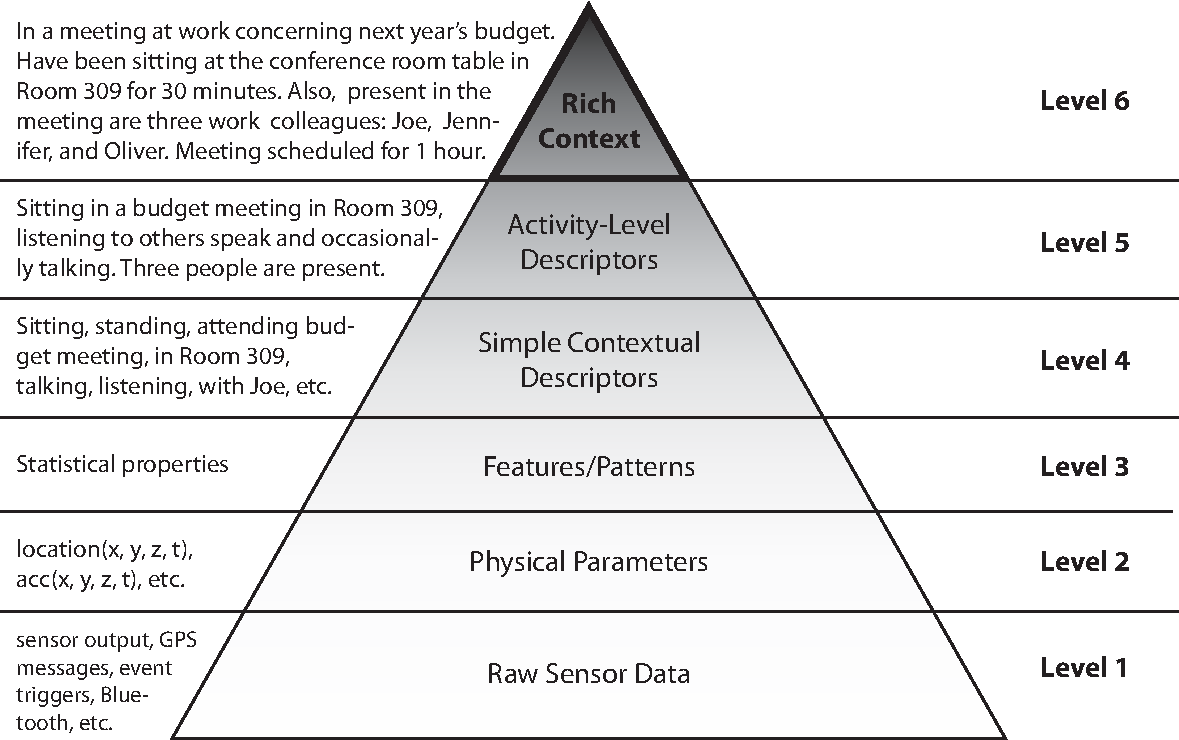
\includegraphics[width=1.0\textwidth]{Images/ContextPyramid4}
  \end{center}
  \caption[The Context Pyramid]{The ``context pyramid'' shows the different levels of processing to build context-aware systems, starting from raw sensor data at the bottom and working up to ``rich context'' at the highest level.}
  % Optional shorter caption in brackets is used in Table of Figures
  % (tof).
  \label{fig:context_pyramid}
\end{figure}
%
Lastly, we can make some general statements about how to process the input data to a context-sensing system. We conceptualize this process as a ``context pyramid'', which was first presented in \cite{pei2013human} and later in \cite{chen_geospatial_2014}. This context pyramid is also shown in Figure~\ref{fig:context_pyramid} below. On the left side is an example of contextual information. At the bottom of the pyramid lies the raw input to the context-sensing system, such as sensor data. The difference between the first and second level in the pyramid is that in Level 2, some ``pre-processing'' of the data may have been performed, such as reference frame transformation or filtering out noise. In the next level of processing, statistical features are extracted from the data, such as mean values or frequency domain features computed from time series data. The distinction between ``pre-processing'' and statistical feature extraction can be a bit blurry in some cases, but generally speaking Level 2 data usually have a clear physical meaning, whereas Level 3 data might have only a mathematical or statistical meaning. Next, Level 4 is achieved after the Level 3 data is subjected to a function or algorithm that performs contextual classification or in some cases regression. This topic will be covered in greater detail in Chapter~\ref{ch:machine_learning}. Level 4 data is in the form of \emph{simple contextual descriptors}, which can be thought of as ``atomic'' elements of context. They each should belong to one of the seven categories described in Section~\ref{sec:framework} above. Then, Level 5 is achieved by combining multiple simple contextual descriptors into an activity-level description of the context, as well as the main pertinent contextual details. Finally, Level 6 combined all available contextual information into a \emph{rich context}. The aim at this level is to approach a description of the context that is indistinguishable from human-written prose. As was the case between Levels 2 and 3, the difference between Levels 5 and 6 can be sometimes blurry. In some context-aware systems there may be fewer processing steps or perhaps more, so even the number of levels should not be taken as dogma. We believe, however, that the general process will always follow the overall trend illustrated in the context pyramid.
%
% \section{Conclusions}
% \label{sec:conclusions}
% %
% In this chapter we have defined the terms context and context awareness and provided a general introduction to the topic. We have attempted to discuss context awareness in an abstract and general way, but we have also pointed out the limitations of such a discussion. Our aim was to give a rough conceptual outline of this research topic, but our strong preference is that context should be discussed with some particular applications in mind, otherwise the subject is simply too broad to provide a general treatment. That being said, there are some general methods that can be employed towards many problems in context awareness, and such methods will be the focus of the next chapter.
\chapter{Machine Learning}
\label{ch:machine_learning}
%
This chapter will provide background on the topic of machine learning, whose role in this thesis was outlined in the introduction chapter. Our preferred definition of ``machine learning research'' was also given in that chapter, but it is worth repeating here:
%
\begin{quote}
Machine learning research seeks to develop computer systems that automatically improve their performance through experience \cite{Mitchell1990}.
\end{quote}
%	
Stated slightly differently, \emph{machine learning} is concerned with developing and analyzing algorithms used by computer systems that automatically improve their performance through experience. An earlier definition, widely attributed to Arthur Samuel, is that machine learning is ``the field of study that gives computers the ability to learn without being
explicitly programmed''\footnote{We have been unable to recover the original source of this quote. Some references cite \cite{samuel1959some}, but the quote is not found in reprints of this article.}. This definition also implies \emph{automatic} learning, but it suffers from the problem that the meaning of ``learn'' is not precisely defined.

As is the case in some fields, the discipline known as ``machine learning'' has drifted somewhat from its original defining aims. This will become more evident later on in this chapter when we describe the major types of machine learning problems that have developed over the past 30+ years.

The chapter is organized as follows. Section~\ref{sec:chess} presents an intuitive example of machine learning in terms of a programming task. Section~\ref{sec:modern-machine-learning} provides an overview of the modern notion of machine learning. Section~\ref{sec:supervised-learning} describes supervised learning, and Section~\ref{sec:unsupervised-learning} describes unsupervised learning. Finally, Section~\ref{sec:ml_concluding_remarks} provides a few concluding remarks on the topic of machine learning.

%Section~\ref{sec:semi-supervised-learning} describes semi-supervised learning, and finally Section~\ref{sec:conclusions-ml} provides concluding remarks.

\section{Computer Chess: An Example Learning Task}
\label{sec:chess}

First, by way of example, we present a classic programming task that could possibly be achieved using machine learning. The task is to create a computer program that can play chess against a human\footnote{Some of the earliest works in machine learning and artificial intelligence involved computer-playing games, such as chess and checkers. See \cite{samuel1959some} \cite{shannon1950xxii} \cite{Turing1953}.}. If the task requirement were \emph{only} to ``play'' chess, then the programming task would be rather trivial and would definitely not require machine learning. The programmer would simply have to encode all the rules of chess (namely how the pieces move and what happens as a result of the moves, such as captures) and then implement a random move selection function that obeys these rules. This program, undoubtedly, would be a very terrible chess player, so we add the additional requirement that the program should try to \emph{beat} a human in chess. This is now a formidable programming task, and one that has been considered by computer scientists at least as far back as Claude Shannon's 1950 paper on the subject \cite{shannon1950xxii}\footnote{For example, according to colleagues of Alan Turing, Turing began considering computer chess during the 1940s.}. Perhaps the most famous chess-playing program was initiated at Carnegie Mellon University in 1985 and later transitioned to IBM, culminating in the computer Deep Blue\textsuperscript{\textregistered} beating the chess master Garry Kasparov in a six-game match-up in 1997\footnote{We note that Kasparov has accused IBM of cheating by letting human players intervene in one of the matches.}. Nowadays, similarly advanced chess programs can run on a personal computer or even a smartphone or tablet. A full literature review of computer chess is beyond the scope of this thesis, but we refer the interested reader to \cite{hsu2002behind} \cite{Spicer2006}, and \cite{Russell2010}. Our intention in this section is to use this chess example as a way to clarify our understanding of the aim of machine learning.

\subsection{Rule-Based Methods}
\label{sec:rule-based}

Let us consider the ways in which we could go about this programming task. One way would be to extend the encoding of the rules of chess to encoding tactics and strategies of great chess masters, attempting to cover as many possible situations in chess, also known as \emph{chess positions}, as we can\footnote{We could have chosen the phrase ``contexts in chess'' rather than ``situations in chess'', thus emphasizing the connection to context awareness, but this seems a bit awkward.}. Basically these strategy rules would instruct the computer what a chess master would do in each of the possible situations. This is essentially the approach that Deep Blue programmers took. Combined with the ability to evaluate hundreds of millions of chess positions per second, these rules eventually succeeded in beating the best human chess players.

This approach, however, hardly fits the above definition of machine learning. In fact, to create Deep Blue required many years of highly ``manual'' work of programmers refining the set of strategy rules, testing the program against human players, and repeating this process. Thus, it falls short of the aim of \emph{automatically} improving performance.

\subsection{A Trivial Chess Learning Program}
\label{sec:trivial-learning}

A trivial \emph{machine learning chess program} could work as follows: The program would simply play against itself and then, at the end of the game, record which side won (or whether there was a draw), as well as the set of moves in the game. Let us call one side \emph{ComputerWhite} and the other \emph{ComputerBlack}, according to convention. As the games are played, \emph{ComputerWhite} would first look-up whether the current position exists in any of the records in the database, and if the record corresponds to a win for \emph{ComputerWhite}, then it would play the next move listed in the record. If multiple winning records exist containing the same position, ComputerWhite should select one of those winning records at random.  Otherwise, it would choose any valid move at random. \emph{ComputerBlack} would do exactly the same, and the program would continue until the game's conclusion. In essence, this program would play many possible chess games, and try to avoid repeating any games that result in a loss or draw\footnote{Under this algorithm, repetition of non-winning games is possible but rather unlikely. Also, it is not guaranteed to play every possible game, though a somewhat simple modification to the algorithm could ensure every game is eventually played.}.

Another very similar version of the program would operate in the same way but allow for the other side to be played by a human. This program would not be very good when the size of the database is small, and furthermore it would learn very slowly because the records in the database would be generated almost completely at random. Nonetheless, it would fit our definition of machine learning, provided that it does not require a human programmer to update the program during or after the learning process.

Such approaches are known as brute force dictionary approaches or \emph{rote learning}\footnote{Note this type of learning is similar to the so-called ``dictionary attack'' used to ``learn'' a log-in password.}. \cite{shannon1950xxii} calculated that such a database (or dictionary) would require roughly 10\textsuperscript{43} entries to record all possible chess positions. Clearly even a very efficient database containing this dictionary would require many ``Google-scale'' data warehouses, and performing look-ups in the database would be prohibitively expensive.  

It is probably fair to say that for most computing tasks, writing a trivial machine learning algorithm is fairly easy, as in the example given above. Therefore, what the discipline of machine learning is mainly concerned about is improving the learning rate and performance rate beyond that of a trivial algorithm, or ideally beyond any state-of-the-art algorithm. There are, of course, other important aspects as well, such as finding algorithms that use minimal amounts of memory or those that can produce simple/efficient models of the learned task. Learning rate and performance, however, are usually the most important aspects of a machine learning algorithm\footnote{Note that performance can be measured in different ways, a topic which we will return to in Section~\ref{sec:supervised-learning}. %TODO: I don't really talk about performance much in this section. Revisit.
In the chess example given above, a good performance metric might be the percentage of games that the computer wins against a randomly selected human player or perhaps the average \gls{fide} rating of the human players it has beaten.}. Lastly, it is important to note that there is no ``one size fits all'' machine learning algorithm. Different algorithms perform better or worse relative to their peers on different problems and learning tasks. This phenomenon has been called the ``no free lunch theorem'', and it has been shown to have a strong mathematical basis \cite{wolpert1996lack}.

\section{Modern Machine Learning}
\label{sec:modern-machine-learning}

In this section, we describe the modern notion of machine learning, which, as we have already alluded to, has developed into something a bit different from what the early pioneers in machine learning had envisioned. That is, today there is a well-established community of machine learning researchers and practitioners whose focus is not entirely the same as what Mitchell, Samuel, or other machine learning pioneers had in mind. Our intention in pointing this out is not to denigrate the discipline of machine learning as a whole but rather to emphasize those aspects of the discipline which fall short of the original goals of machine learning. 

Let us first present a few other definitions of machine learning found in recent textbooks on the subject:
%
\begin{quote}
Machine learning is programming computers to optimize a performance criterion using example data or past experience \cite{alpaydin2014introduction}.
\end{quote}
%

This definition appears quite close to that of \cite{Mitchell1990}, if we assume that ``example data'' can be generated automatically. This may be true in some cases, but in most methods described in \cite{alpaydin2014introduction}, the example data are data that have been manually labeled with the ``correct'' value relative to the performance criterion that is to be optimized. Although programs using such methods can improve their performance by obtaining more example data, if the example data cannot be generated automatically, then the method would fall short of \cite{Mitchell1990}.

Another recent definition is given by \cite{Murphy2012}, which defines machine learning as:
%
\begin{quote}
a set of methods that can automatically detect patterns in data, and then use the uncovered patterns to predict future data, or to perform other kinds of decision making under uncertainty (such as planning how to collect more data!).
\end{quote}
%
This definition includes the ``automatic'' aspect, similar to \cite{Mitchell1990}, although we prefer the definition of \cite{Mitchell1990} due to its simplicity.

We note that some books on machine learning (e.g. \cite{bishop2006pattern}) omit to precisely define machine learning, perhaps because it has come to encompass many diverse methods. One book goes so far as to explicitly refuse to define machine learning in any principled way:
%
\begin{quote}
the kind of learning techniques explained in this book...are called machine learning without really presupposing any particular philosophical stance about what learning actually is \cite{witten2005data}
\end{quote}
%

% Despite these disagreements as to the precise definition of machine learning, most experts agree on the classification of machine learning methods into two main categories of 

% This group of methods is known as \emph{supervised learning}, and it will be discussed further in Section~\ref{sec:supervised-learning}. Similarly, many of the other methods described in \cite{alpaydin2014introduction} are focused on discovering structure in a set of data. The ``learning task'' is to find the structure in a given set of data, but this structure is inherently dependent on the dataset itself, so this task is not a machine learning task in the sense of \cite{Mitchell1990}. Such methods fall under the category known as \emph{unsupervised learning}, which will be discussed in greater detail in Section~\ref{sec:unsupervised-learning}.

Mitchell, on the other hand,  also provides a precise definition of the concept of learning in the context of machine learning:
%
\begin{quote}
A computer program is said to \emph{learn} from experience \emph{E} with respect to some class of tasks \emph{T} and performance measure \emph{P}, if its performance at tasks in \emph{T}, as measured by \emph{P}, improves with experience \emph{E} \cite{Mitchell1997}.
\end{quote}
%
%
%

% adding economic aspects to this definition, i.e. cost of learning and value produced by tasks...?

Continuing with formalisms, many learning tasks can be expressed in terms of learning a mathematical function between the inputs to the task and the desired outputs. In other words, the learning task is to find some optimal mapping between the inputs and the possible outputs. This can be expressed as follows:
%
\begin{equation}
f : \mathbf{x} \rightarrow y
\end{equation}where $f$ is a function, $\mathbf{x}$ is a vector of inputs of arbitrary dimension, and $y$ is an output with $y \in Y=\{y_1, y_2,...y_m\}$, corresponding to the set of all possible outputs (which may or may not be finite). The function $f$ is also called a model in many textbooks on machine learning.

A simple physical example of a function or model would be a spring scale that maps a displacement length to a weight. In this example, we know from Hooke's law that the function is linear and given by the spring constant $k$, but in many problems the form of the function is unknown, as well as its parameters.

Machine learning techniques differ mainly in how they express and learn this unknown function $f(\mathbf{x})$ and also the form in which $y$ (and therefore the set $Y$) are expressed. For example, $Y$ may be a continuous range or a finite, discrete set. When the learning task involves a continuous-valued output value, it is called \emph{regression}. The spring example given above would be a regression problem. In some cases, the desired output may also be a vector of different values, representing different physical quantities (e.g. the height and weight of a person).

When the output valuable is discrete, we call it \emph{classification}, since the possible values generally represent different \emph{classes} or categories. One example would be the problem of determining whether a person is male or female based on voice recordings. This example highlights the fact that for some machine learning problems, it may be well accepted that the problem cannot be solved perfectly\footnote{One can imagine that for some individuals, voice recordings may not be enough to determine gender.}. Such problems may be best represented in probabilistic form.

In many cases, a machine learning algorithm actually estimates the conditional probability $p(y|\mathbf{x})$. This distribution, $p(y|\mathbf{x})$, may be intrinsically important to the application at hand, or it may be an intermediate step towards determining the most likely value of $y$ according to:
%
\begin{equation}
y = \argmax_{y \in Y} p (y|\mathbf{x})
\end{equation}
%
This is known as the \gls{map} estimate of $y$. One of the benefits of estimating $p(y|\mathbf{x})$, however, is that provides a measure of the confidence of the output $y$.

Algorithms designed to learn $p(y|\mathbf{x})$ are known as \emph{discriminative} approaches. An alternative approach is to first learn a model of the joint probability $p(y,\mathbf{x})$ and then condition on $\mathbf{x}$ to derive $p(y|\mathbf{x})$. These are known as \emph{generative} approaches.



Apart from the distinctions regression vs.\ classification and discriminative vs.\ generative, there are two main categories of machine learning techniques, based on how the unknown function $f$ is learned or approximated. The first category is known as \emph{supervised learning}. In supervised learning, a ``trainer'' supervises the learning process. The goal is essentially then to transfer the knowledge of the trainer or supervisor in the form of a mathematical or computerized model. More details on supervised learning will be covered in Section \ref{sec:supervised-learning}. The other main category is known as \emph{unsupervised learning}. In unsupervised learning, the learning process is not guided in any significant way. The goal is essentially to uncover patterns that are implicit in the data but unobvious.   More details on unsupervised learning will be covered in Section~\ref{sec:unsupervised-learning}.

From this point forward in this thesis, we will drop the distinction between the modern popular notion of machine learning and the earlier meaning of \cite{Mitchell1990} and focus mainly on the mainstream meaning and the main techniques from machine learning. Whenever necessary, we will use the term \emph{automatic learning} to refer to the subset of machine learning where performance improvements take place without requiring any human intervention.
%
\section{Supervised Learning}
\label{sec:supervised-learning}
%
As stated above, supervised learning uses a ``trainer'' to supervise the learning process. In most cases, the trainer has encoded his or her knowledge in the form of \emph{labeled data}, also known as \emph{training data} or a \emph{training set}. In terms of the function $f$ expressed above, the training consists of input-output pairs $\mathcal{D} = \{(\mathbf{x}_i, y_i)\}_{i=1}^N $, where $\mathbf{x}_i$ is an input of arbitrary dimension, $y_i$ is a ``labeled'' output, and $N$ is the number of training samples, such that $\mathcal{D}$ provides \emph{examples} of values of the function $y = f(\mathbf{x})$. In simple terms, the training data provide sample input data that are \emph{labeled} with the correct or desired output.

It is usually the case that the training data does not exhaustively define the unknown function $f$. If, however, certain assumptions can be made about the function, then the function might be fully specified by a finite set of training data. In the simplest case, where $f$ is linear and $\mathbf{x}$ is one-dimensional, then only two training samples are needed to specify the relationship between $\mathbf{x}$ and $y$\footnote{Recall that two points define a straight line.}. Most practical examples of machine learning algorithms are more complicated due to (1) higher dimensionality, (2) non-linearity, and (3) error present in the training data.

Let us consider a simple example from the domain of context awareness. Suppose we have a smartphone application that needs to know whether the user is walking, running, or standing still (i.e. static). We refer to these as \emph{mobility contexts}. The smartphone has a GPS receiver that can record the user's position and speed, and it also has a three-axis accelerometer that can measure acceleration. Instead of using the raw accelerometer signal, we define a feature from the accelerometer data, known as \emph{dynamic acceleration}:
%
\begin{equation}
a_d = var(\{\sqrt{a_{xi}^2 + a_{yi}^2 + a_{zi}^2}\}_{i=1}^N\,)
\end{equation}
%
where $var(\cdot)$ is an operator that computes the variance over some time series of data (e.g.\ one second of acceleration data); $a_{xi}$, $a_{yi}$, $a_{zi}$ are the accelerations in the $x$, $y$, and $z$ directions, respectively, for some given time epoch $i$; and $N$ is the number of samples in the time series.

A researcher, Mary, has painstakingly collected a dataset for developing a context-aware application and labeled whether she was walking, running, or standing still. Some sample data are shown in Table~\ref{table:data-from-phone} below, consisting of two dimensions of input data and the labeled output. In order to keep the size reasonable, only 35 data samples are shown in the table. In Figure~\ref{fig:data-from-phone-supervised}, similar data are plotted, but now we include 1000 samples from each class.

Based on this figure, several observations can be made. We clearly see three clusters of data, corresponding to the three mobility contexts. The cluster corresponding to the ``static'' context is well separated from the other two, but in the case of the ``walking'' and ``running'' contexts, there is some overlap. Another important observation is that in the ``walking'' data, some of the values for speed are very close to 0 m/s. This could be due to errors in the data (i.e. the data from the GPS receiver might have some error) or labeling errors made by Mary. Similarly, the static data contain many points where the speed is non-zero. It is very common with this type of data that some labeling errors are present in the training set. For example, at the transition points between the walking and static contexts, it is difficult to accurately label which data corresponds to ``walking'' and which corresponds to ``static''\footnote{One technique to avoid such labeling errors is to remove these transition points entirely from the training set.}.
\begin{table}
\caption[Example data for supervised learning]{Example data for supervised learning. The data consist of two-dimensional input data from smartphone sensors and a labeled output class.}\label{table:data-from-phone}
\centering
\begin{tabular}{lccc}
\hline\noalign{\smallskip}
\textbf{ID} & \textbf{Speed (m/s)} & \textbf{Dyn. accel. (m\textsuperscript{2}/s\textsuperscript{4})} & \textbf{Label}\\
\hline\noalign{\smallskip}
1 & 2.56 & 21.10 & walking\\
2 & 0.94 & 28.78 & walking\\
3 & 1.24 & 31.22 & walking\\
4 & 2.99 & 36.66 & walking\\
5 & 1.24 & 36.43 & walking\\
6 & 0.64 & 29.88 & walking\\
7 & 0.73 & 34.13 & walking\\
8 & 1.68 & 28.56 & walking\\
9 & 2.72 & 32.96 & walking\\
10 & 1.82 & 38.57 & walking\\
11 & 2.10 & 30.70 & walking\\
12 & 2.80 & 49.59 & running\\
13 & 4.01 & 47.41 & running\\
14 & 3.10 & 61.96 & running\\
15 & 1.98 & 54.44 & running\\
16 & 2.33 & 53.92 & running\\
17 & 5.48 & 44.49 & running\\
18 & 4.14 & 52.38 & running\\
19 & 2.69 & 52.85 & running\\
20 & 4.73 & 44.02 & running\\
21 & 1.22 & 48.76 & running\\
22 & 4.88 & 47.78 & running\\
23 & 0.40 & 2.89 & static\\
24 & 0.92 & 0.92 & static\\
25 & 0.36 & 1.48 & static\\
26 & 1.16 & 3.37 & static\\
27 & 0.00 & 5.76 & static\\
28 & 0.28 & 3.27 & static\\
29 & 0.60 & 0.70 & static\\
30 & 0.45 & 2.97 & static\\
31 & 1.44 & 1.79 & static\\
32 & 0.11 & 1.45 & static\\
33 & 1.36 & 1.51 & static\\
34 & 1.06 & 0.03 & static\\
35 & 0.81 & 1.28 & static\\
\hline\noalign{\smallskip}
%
\end{tabular}
\end{table}
%
In this example, the goal of supervised learning would be to find a function $f$ that maps the input data $\mathbf{x}_i = (speed^i,a_d^i)$ to the correct output class, i.e.  $y_i \in \{`walking\textrm',$  \linebreak$`running\textrm',$ $`static\textrm'\}$, such that the number of errors are minimized. In this context, errors could be defined as input data that are mapped to the wrong output class, also known as misclassifications.
%
\begin{figure}

\begin{center}
    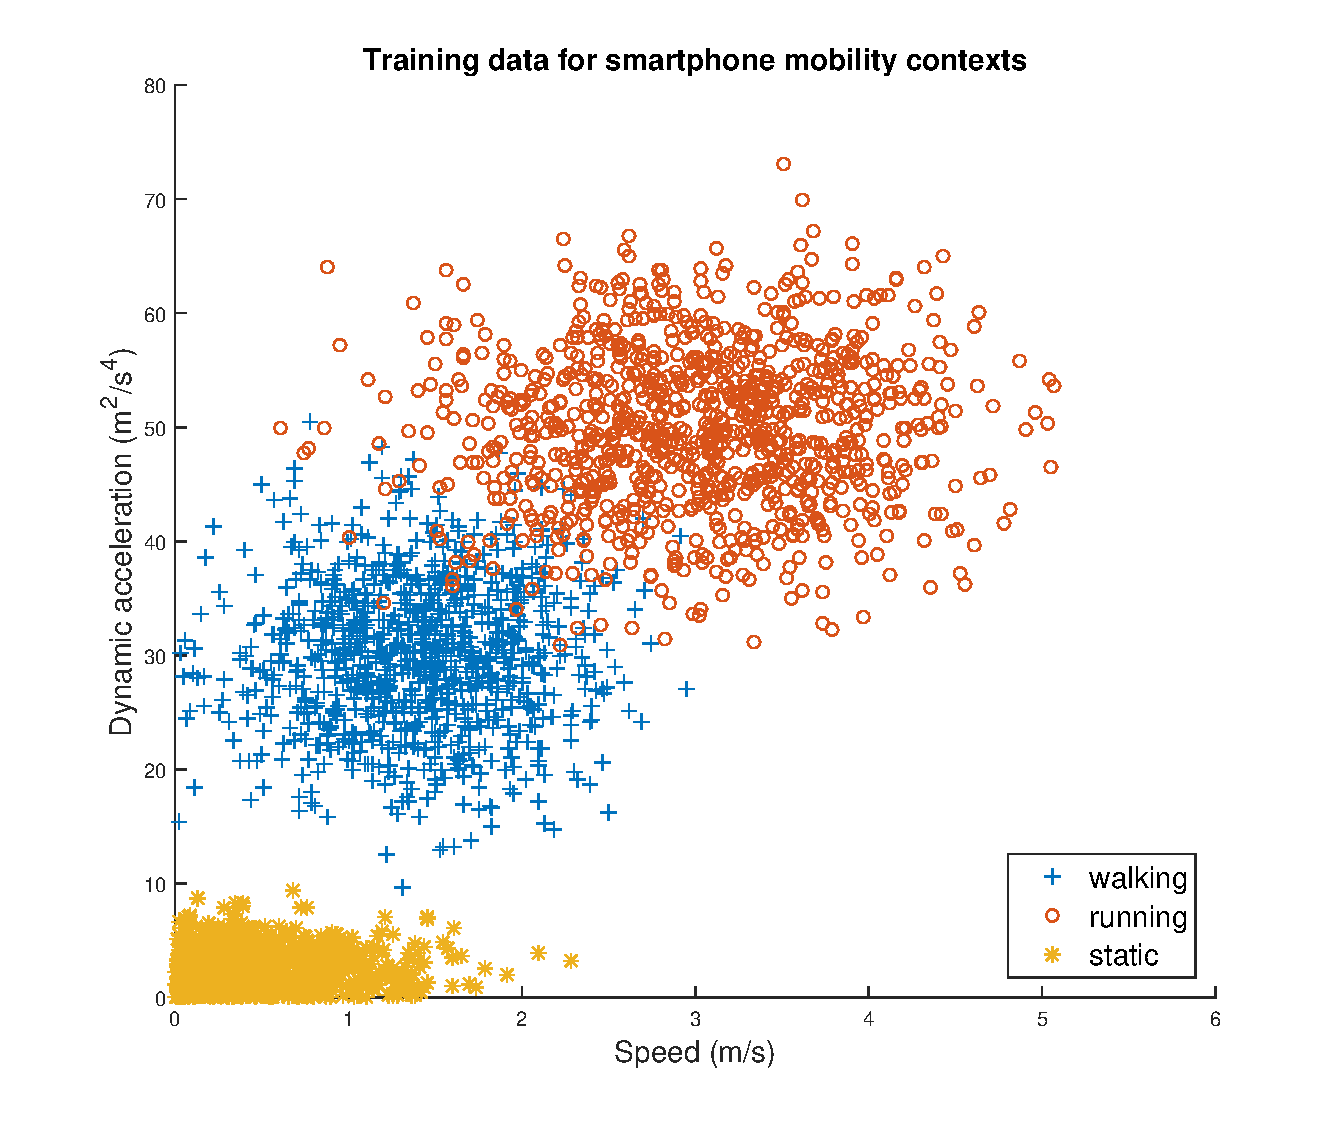
\includegraphics[width=1.0\textwidth]{Images/figChapter3-1}
  \end{center}
  \caption[Training data for supervised learning]{Example training data for supervised learning. The data are similar to those shown in Table~\ref{table:data-from-phone}. Note the partial overlap between the ``walking'' and ``running'' classes.}
  \label{fig:data-from-phone-supervised}
\end{figure}

Three important interrelated concepts should now be introduced: \emph{generalization}, \emph{underfitting}, and \emph{overfitting}. Generalization refers to the idea that supervised learning should ``generalize'' beyond the specific examples given in the training set. In other words, the goal is not simply to map the inputs to the outputs for the given training set but rather to find a mapping function that works well on some yet unseen data. If the goal were simply to fit a function to the training set, then it would be trivial to write a function that performs with zero errors (e.g. a simple lookup table would do the job).

%Ideally the function should cover the entire input space.

Overfitting refers to the situation where the supervised learning algorithm has produced a mapping function that follows the training data in too much detail. Keep in mind that every training set is somehow incomplete and imperfect. If the training results in a function that does not properly take into account the gaps and the noise in the training data, then it will \emph{overfit} the training data and will not generalize well.

It is also possible that a mapping function \emph{underfits} the training data. This usually means that the mapping function is overly simple, for example, using a linear model for data that is inherently non-linear. Therefore, good generalization lies in between the two extremes of underfitting and overfitting. The goal of learning is more precisely defined as minimizing the \emph{generalization error}, which is the average error rate that will be produced by any future data, and this means finding a model that neither overfits nor underfits. Of course, it is difficult to estimate the true generalization error. The most common approach is to use an independent \emph{test set}. A test set is simply another labeled dataset that is not used in the learning process but is reserved for estimating the generalization error after learning has already taken place.

A test set provides a way to measure the generalization error and see whether any overfitting or underfitting is occurring, but the question remains: How does one determine the right type of function or model to fit to the training data? This process is known as \emph{model selection}. In model selection, we siphon off yet another portion from the training set, known as the \emph{validation set}. The model selection process then proceeds as follows:
%
\begin{enumerate}
\item Choose a hypothesis set $\mathpzc{H}$ containing different hypothesis function types to be used in model selection. This hypothesis set can be of one particular function class, such as the set of all linear functions or can be of several different classes. The goal is to include within the hypothesis set a class of functions that match well with the underlying data under investigation. This is , however, non-trivial and may require some precursory \emph{data exploration}.
%
\item Given the hypothesis set $\mathpzc{H}$, for each hypothesis class $\mathpzc{H}_i \in \mathpzc{H}$, use the training set $\mathcal{D}$ to find the best function $h_i \in \mathpzc{H_i}$.  For example, if $\mathpzc{H}_i$ is the set of all linear functions of the form $h(x) = a * x + b$, then this step is equivalent to finding the parameters $a$ and $b$ that best match the training data, according to some linear regression estimator, e.g. the least squares estimator.
%
\item Now we have a set of fitted functions, each from a different hypothesis class. That is, for each $\mathpzc{H}_i$, we have a corresponding fitted function $h_i$. Let us denote these as $\mathpzc{H}_{best-in-class} = \{h_i\}_1^N$, where $N$ is the number of hypothesis classes. The next step is to choose the best $h_i$ from this set. For this, we use the validation set to measure the error rate and choose the function with the lowest error, which we denote $h_{best}$, and its hypothesis class is denoted by $\mathpzc{H}_{best}$.

\item Finally, fit a new function $h_i \in \mathpzc{H}_{best}$ using the training set plus the validation set, and measure its  error using the test set. Since the test set was not used in the learning process, the resulting error rate can be considered an estimate of the generalization error.
\end{enumerate}
%
Depending on the amount of labeled data available, and the complexity of the underlying structure in the data, it may be necessary to repeat this process with different divisions of the labeled data into the respective training set, validation set, and test set. The standard technique for this repetition process is known as \emph{cross-validation}. Due to space limitations, we will not cover cross-validation in detail, but it was employed in [P3] and [P4].%TODO.

So far we have discussed general concepts in supervised learning but not any specific algorithms. Several examples of supervised learning algorithms will be described in [P2].
%
\section{Unsupervised Learning}
\label{sec:unsupervised-learning}
Unsupervised learning is, in many ways, quite similar to supervised learning, except that there are no labeled data. In other words, there are only input data, and the goal is to learn something about the structure or patterns in the input data. In this way, unsupervised learning is very similar to traditional statistical methods, where the goal is to infer a statistical model from a set of data. Many unsupervised learning methods, such as density estimation, come straight from statistics. Others differ only in the name or some other superficial characteristics. Especially in recent years, there are large overlaps between statistics research and unsupervised learning research\footnote{This is also true to a certain extent in supervised learning, but the similarity is more striking in unsupervised learning.}.

\begin{figure}
  \begin{center}
    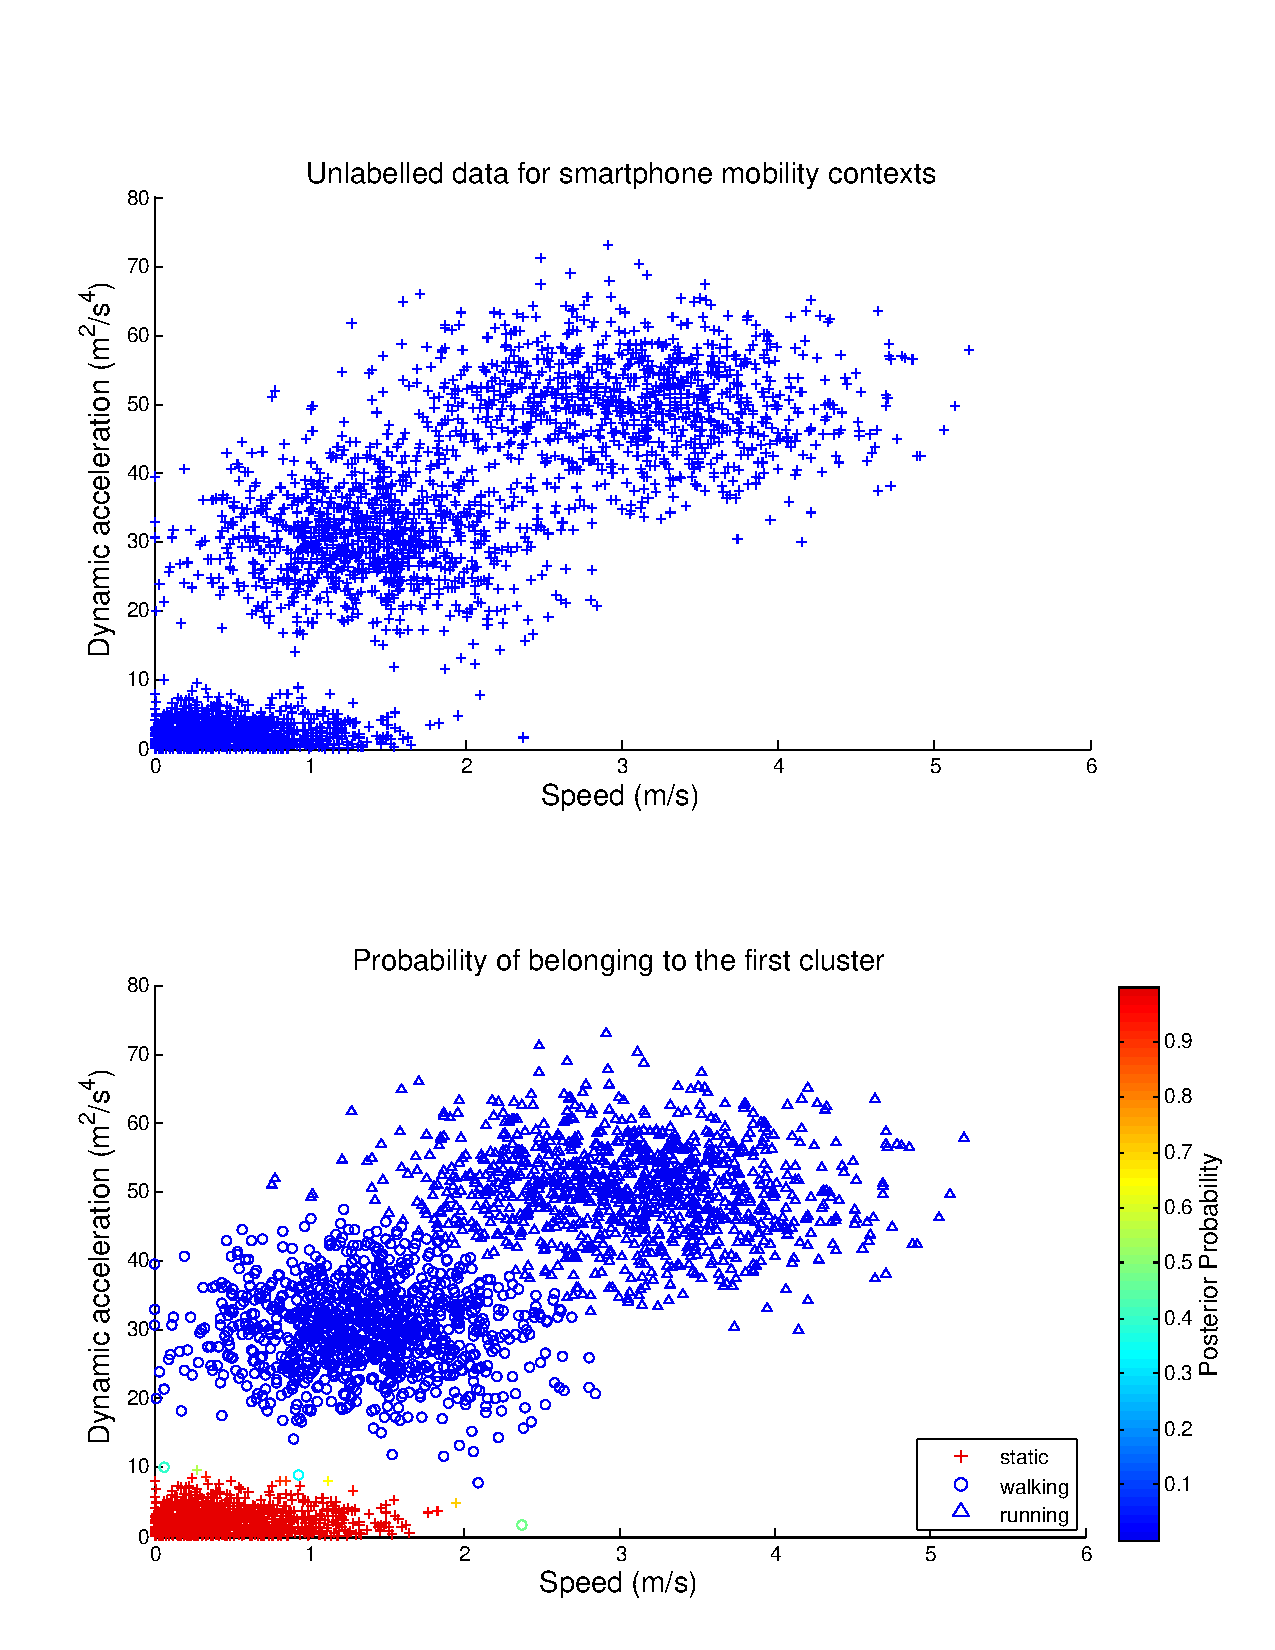
\includegraphics[width=1.0\textwidth]{Images/figChapter3-2}
  \end{center}
  \caption[Input data for unsupervised learning and one clustering result]{The top plot shows example input data for unsupervised learning. In contrast to Figure~\ref{fig:data-from-phone-supervised} no labels are available. The bottom plot shows one result from the EM-based clustering. The color of the points shows the posterior probability that the points belong to the first component in a GMM. Data labels are shown strictly for demonstration purposes. In a real situation, no such label would be available to interpret the unsupervised learning result.}
  \label{fig:data-from-phone-unsupervised}
\end{figure}

Consider again the data presented in Table~\ref{table:data-from-phone} and Figure~\ref{fig:data-from-phone-supervised}. Suppose Mary had not gone to the trouble of labeling the data with the actual mobility context associated with each data sample. We would have then only a two-dimensional dataset of input data, and we could make a similar plot as Figure~\ref{fig:data-from-phone-supervised}, except the legend would be missing and we would also not have the information necessary to label the samples with different colors as in Figure~\ref{fig:data-from-phone-supervised}. The top part of Figure~\ref{fig:data-from-phone-unsupervised} shows such a plot.
%

One unsupervised learning task would be to identify different clusters or groups present in the data. Depending on the data and the application, it may or may not be apparent how many clusters are inherently present in the data, so the number of clusters may also be a parameter to determine as part of the unsupervised learning task. There are a plethora of different unsupervised learning algorithms available in the literature that perform clustering. Possibilities include k-means clustering \cite{hartigan1979algorithm}, \acrshort{optics} \cite{Ankerst:1999:OOP:304181.304187}, and the \gls{em} algorithm \cite{dempster1977maximum}. In particular, the EM algorithm has its roots in statistics and can fit observed data to an arbitrary statistical model.

To provide an example of clustering, we used the EM algorithm to fit a \gls{gmm} to the data that we have previously seen in the top half of Figure~\ref{fig:data-from-phone-unsupervised}. A GMM is of the form:
%
\begin{equation}
 p(\mathbf{x}|\Theta) = \sum\limits_{k=1}^K \pi_k \phi_k(\mathbf{x}; \boldsymbol{\theta}_k)
\end{equation}
%
where $\mathbf{x}$ is a random vector, $K$ is the number of components in the mixture model, $\phi_k(\mathbf{x}; \boldsymbol{\theta}_k)$ are normal distributions with parameters $\boldsymbol{\theta}_k = (\boldsymbol{\mu_k}, \mathbf{\Sigma_k})$, $\pi_k$ are mixing weights satisfying $\pi_1 + ... + \pi_K = 1, \pi_k \geq 0$, and $\Theta = \{\pi_1,...,\pi_K,\theta_1, ..., \theta_K\}$ is the complete set of model parameters\footnote{The notation used for the GMM is similar but not identical to that given in \cite{bilmes1998gentle}.}.

The EM algorithm itself is a widely-used iterative algorithm used to find the \gls{mle} of the model parameters (which we denote with $\Theta$ as above) for an underlying distribution $p(\mathbf{x}|\Theta)$ used to model a given dataset, which we denote as $\mathcal{D} = (\mathbf{x}_1,..., \mathbf{x}_N)$ \cite{bilmes1998gentle}. The MLE is obtained by maximizing a function $Q$ equal to the expected value of the log-likelihood $\mathcal{L}(\Theta|\mathcal{D},\mathcal{Y})$, given the observed data $\mathcal{D}$ and the current parameter estimates $\Theta^{(i-1)}$:
%
\begin{gather}
  Q(\Theta,\Theta^{(i-1)}) = E[\log \mathcal{L}(\Theta|\mathcal{D}, \mathcal{Y})|\mathcal{D},\Theta^{(i-1)})]
     = E[\log p(\mathcal{D}, \mathcal{Y}|\Theta)|\mathcal{D},\Theta^{(i-1)})]
\end{gather}
%
where $\mathcal{Y} = (y_1, ..., y_N)$ is a vector of latent variables that indicate to which component of the GMM a given data sample $\mathbf{x}_j$ belongs. The latent variables can be expressed in various ways, but perhaps the simplest expression is that $y_j = k$ when $\mathbf{x}_j$ belongs to component $k$. In the above equation $i$ indexes the current iteration interval of the algorithm, so $\Theta^{(i-1)}$ represents the parameter estimate from the previous iteration (or the initial estimate, if $i=1$).

Before applying the EM algorithm to find the parameters $\Theta$ of a GMM, one must decide on the number of components $K$ to incorporate into the GMM. As we shall see, each component $k$ in the model will correspond to a cluster in the final clustering result; thus, this step is, in practice, the same as determining the number of clusters, and we can consider $K$ to be a hyperparameter in the estimation problem.

Various methods can be used to determine the best value for $K$. For low-dimensional data, a practical method is to simply plot the data (as we did in the top half of Figure~\ref{fig:data-from-phone-unsupervised}) and try to visualize the inherent number of clusters. For high-dimensional data ($D>3$), this simple approach is not necessarily adequate, nor does it support the goal of automation described earlier. Therefore, a more sophisticated, systematic approach is preferred, such as the one described in \cite{vlassis2002greedy}. For this example in the interest of space, we assume that the choice of $K$ is already clear, and for these data $K=3$ seems to be a reasonable choice.

The next step is simply to apply the EM algorithm to determine the parameters $\Theta$ of our three-component GMM. A detailed description of the EM algorithm is beyond the scope of this thesis, but here we provide a brief overview.

First, EM requires an initial estimate of $\Theta$, and various initialization techniques to provide sensible initial estimates can be found in the literature . A simple approach is to use the given dataset $\mathcal{D}$: e.g. select $K$ random samples to initialize $\boldsymbol{\mu_k}$ and use the covariance matrix of $\mathcal{D}$ for each of the initial $K$ covariance matrices $\boldsymbol{\Sigma_k}$ \cite{Smyth2015}.

After initialization, the algorithm then alternates between computing an expectation function (known as the E-step) and finding the parameters $\Theta$ that maximize this function (known as the M-step). At each E-step, the algorithm calculates a new $Q(\Theta,\Theta^{(i-1)})$. In the M-step, an updated estimate $\Theta^{(i)}$ of the parameter set is obtained by maximizing $Q(\Theta,\Theta^{(i-1)})$, according to:
%
\begin{equation}
 \Theta^{(i)} = \argmax_\Theta{Q(\Theta,\Theta^{(i-1)})}
\end{equation}
%
The algorithm terminates when $Q(\Theta,\Theta^{(i-1)})$, evaluated at $\Theta$ = $\Theta^{(i)}$, converges towards a maximum value (i.e. improvement is below some threshold value $\epsilon$).

Finally, once the parameters $\Theta$ are estimated, we can determine the posterior probability that a data sample $\mathbf{x}_j$ belongs to a particular component $k$ of the GMM, according to its so-called ``membership weight'' \cite{Smyth2015}:
%
\begin{equation}
  w_j^k = p(y_j = k|\mathbf{x}_j, \Theta) =  \frac{p_k(\mathbf{x}_j|\theta_k) \pi_k}{ \sum_{m=1}^K p_m(\mathbf{x}_j|\theta_m) \pi_m }
\end{equation}
%
Recall that each component of the GMM corresponds to a cluster, and therefore the membership weight for a given $k$ is the posterior probability that the data sample belongs to cluster $k$. The bottom half of Figure~\ref{fig:data-from-phone-unsupervised} and Figure~\ref{fig:data-from-phone-unsupervised2} show the posterior probabilities for our example data, corresponding to membership in each of the three clusters. Note that a dividing line between membership in each cluster can be drawn where the posterior probability reaches 0.5.
%
\begin{figure}
  \begin{center}
    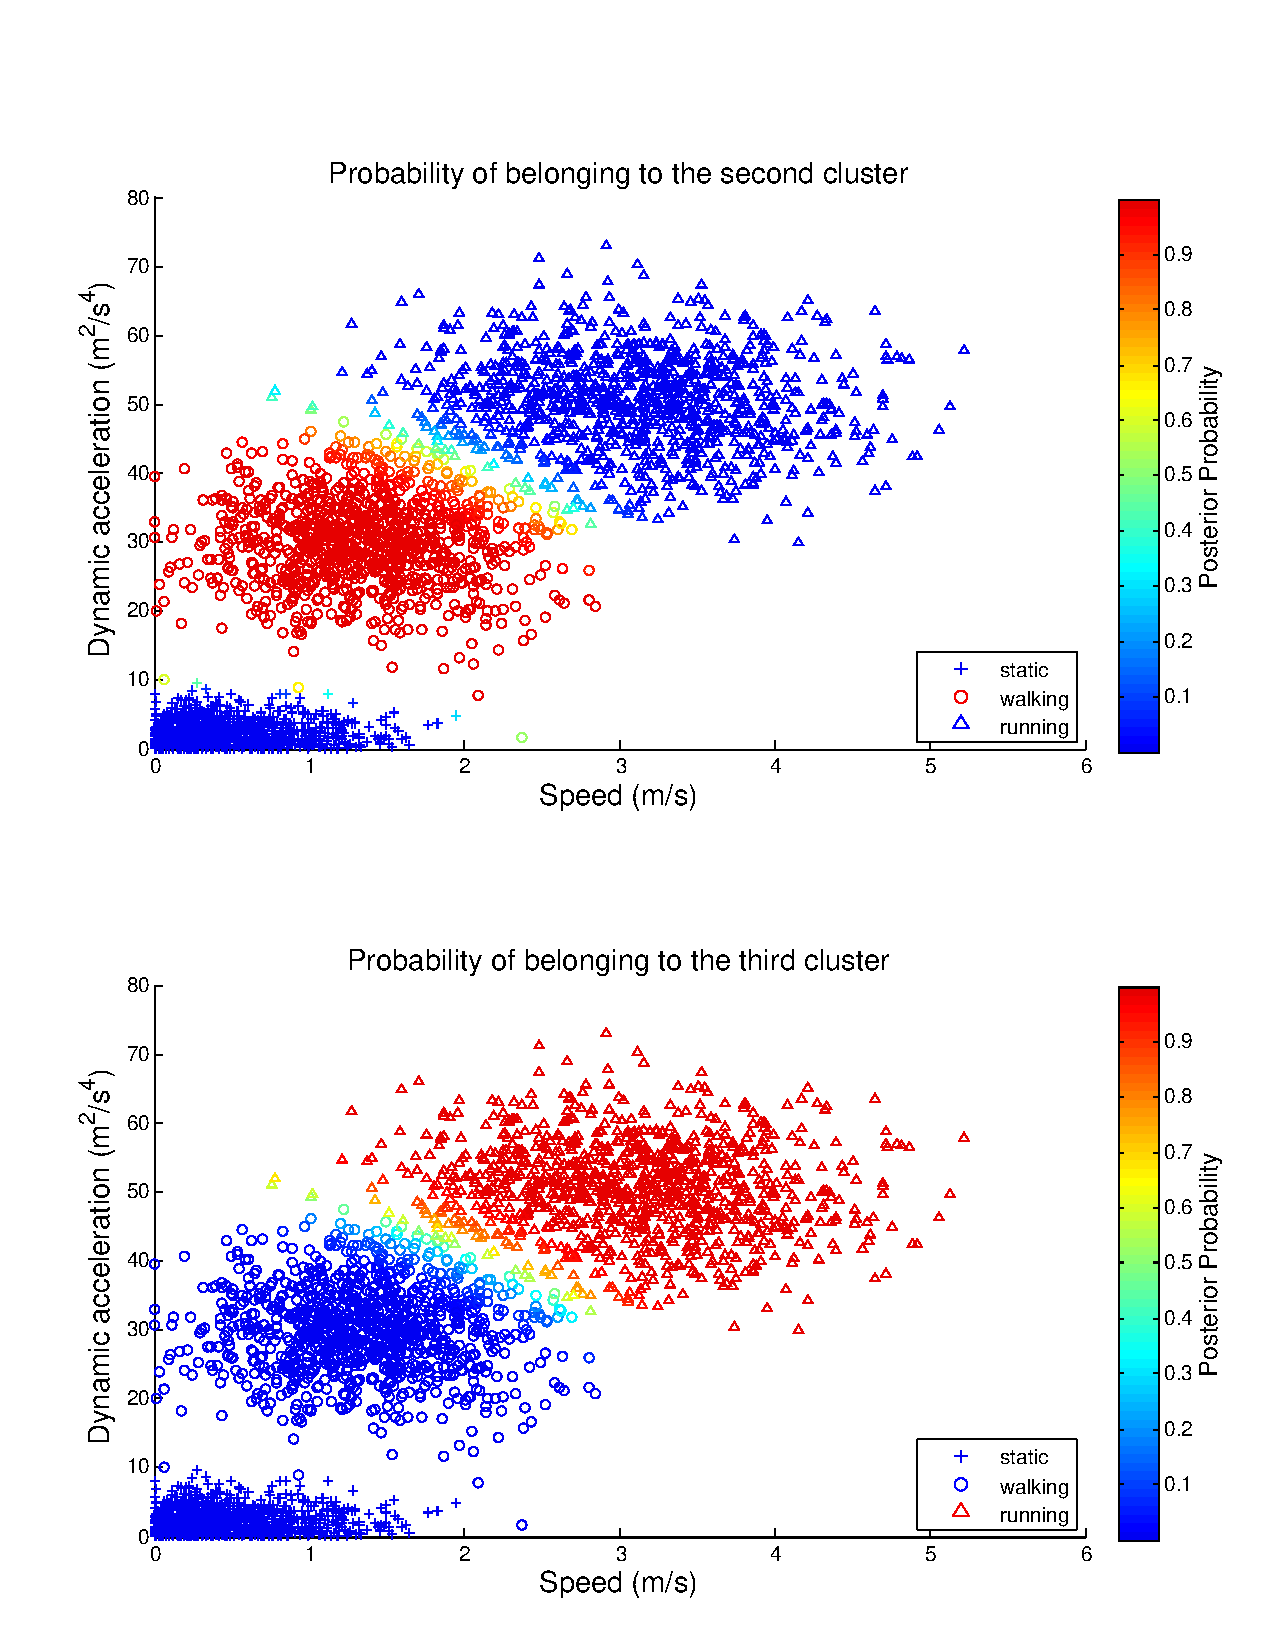
\includegraphics[width=1.0\textwidth]{Images/figChapter3-3}
  \end{center}
  \caption[Further results from unsupervised learning]{These two plots continue the results presented in Figure~\ref{fig:data-from-phone-unsupervised}. The coloring used in the top plot shows the posterior probabilities that the points belong to the second component in a GMM, whereas the bottom plot shows the same for the third component. As in Figure~\ref{fig:data-from-phone-unsupervised}, the data labels are shown strictly for demonstration purposes.}
  \label{fig:data-from-phone-unsupervised2}
\end{figure}
%
%\section{Semi-supervised Learning}
%\label{sec:semi-supervised-learning}

\section{Concluding Remarks}
\label{sec:ml_concluding_remarks}

Machine learning is clearly a wide topic covering many different concepts and techniques. Our purpose in this chapter was to introduce the most important concepts and to elucidate how machine learning can be used to endow computing systems with context awareness. Further examples and details will be given in the included publications. We have emphasized the role of training data in supervised learning, but we have also demonstrated how a similar result can be achieved through the use of unsupervised learning.

%If the task is formulated in a slightly different way, however, it could be truly considered a machine learning task. We formulate this task as follows:
%
%Let P be a process whose state can be characterised by a value S, which is not directly measurable by any known means. Furthermore, let P produce a set of N-dimensional data X, which can %be measured (e.g. by a set of sensors). Lastly, to keep things simple, let there be a steady-state but unknown relationship F between S and X, such that F(X) = S. 
\chapter{Overview of Publications}
\label{ch:overview_of_publications}

This chapter provides an introduction and overview to the five publications included in this compendium thesis. Two of the publications, [P1] and [P2], are excerpted from the book \emph{Geospatial Computing in Mobile Devices}, published by Artech House in 2014. Two others, [P3] and [P4], were published in the peer-reviewed open access journal \emph{Sensors}. The final publication [P5] was published in the 2014 Proceedings of the \gls{plans}, jointly organized by the \gls{aess} and the \gls{ion}. AESS is an affiliate society of the \gls{ieee}.

The remainder of this chapter is organized as follows: Section~\ref{sec:summary_of_publications} briefly summarizes the publications. Section~\ref{sec:relating_to_research} maps the included publications to the overall research goals presented in this thesis. Section~\ref{sec:author_contributions} describes the author's contributions to each publication. 

\section{Summary of Publications}
\label{sec:summary_of_publications}

Next, we briefly summarize the included publications.

\textbf{[P1]} presents the concept of context awareness at a conceptual level, as well as tracing its historical development. It presents a conceptual framework for describing context, adapted from the seven elements of circumstance, first introduced by Hermagoras of Temnos in the 2nd Century BC. Our motivation was that existing literature on context awareness did not provide any comprehensive, simple, yet flexible framework for describing context. The publication also aims to show at a practical level how different aspects of context awareness can be implemented in a mobile device. Examples are given for the Android \gls{os}.

\textbf{[P2]} presents the concept of contextual reasoning, which is defined as the process of forming higher level inferences about context from lower level information. From this definition, we elaborate a conceptual model of contextual reasoning, which we call the ``context pyramid''. The context pyramid describes contextual reasoning as a series of processing steps at different levels, starting with raw sensor data at the base of the pyramid and working up to the peak of the pyramid, where rich context is realized. We argue that machine learning is the primary technique used for contextual reasoning, and we provide several examples of different machine learning techniques, such as  na\"{i}ve Bayes' classifiers, \gls{hmm}, Bayesian Networks, and \gls{svm}.

\textbf{[P3]} combines indoor positioning technologies and smartphone sensors to detect different human activities in an office environment. We provide a real-world implementation of the context pyramid on a smartphone, resulting in a contextual reasoning capability, which we call the ``cognitive phone''. The key technologies we utilize include ubiquitous positioning, motion recognition, and human behavior modeling. We combine these technologies into a single probabilistic model, which we call the LoMoCo (Location-Motion-Context) model. In this thesis, we demonstrate the feasibility of the fifth level in the context pyramid---Activity-Level Descriptors. Also, the location accuracy we achieved using WLAN-based positioning is about 2--5 meters, depending on the type of space. For motion recognition, we evaluated several different supervised learning techniques, such as decision trees and \gls{lda}, but the best performance was achieved using a \gls{lssvm} classifier with an average recall rate of 92.9\%.

\textbf{[P4]} investigates the use of smartphone sensors, geospatial information, and machine learning to sense mobility contexts, including walking, running, driving and using a bus or train. Our aim was to evaluate techniques that could be used  in real-time or  near-real-time (<5 s). We also measured the computational complexity of the resulting classifiers because this impacts smartphone battery usage. We investigate a wide range of supervised learning techniques for
classification, including decision trees (DT), support vector machines (SVM), naive Bayes classifiers (NB), Bayesian networks (BN), \gls{lr}, artificial neural networks (ANN) and several instance-based classifiers (\acrshort{kstar}, \acrshort{lwl} and \acrshort{ibk}). We performed feature selection to identify the most important features from our dataset for detecting mobility context. Finally, we focus on the best performing classifier, RandomForest, which is a type of ensemble decision tree algorithm. We tune its parameters to find the optimal performance. This resulted in an average recall rate above 97.5\% after tuning. We measure computational complexity in terms of \gls{cpu} time needed for classification to provide a relative comparison between the algorithms in terms of battery usage requirements. As a result, we are able to rank the classifiers from lowest to highest complexity as follows: SVM, ANN, LR, BN, DT, NB, IBk, LWL and KStar. The RandomForest algorithm, although it does not generate the simplest classifier in terms of computational cost, provides the best performance with reasonable complexity.
% test these results for statistical significance

\textbf{[P5]} examines the feasibility of an ice-aware maritime route optimization algorithm and presents a novel method for such purposes. Our aim is to increase the safety and efficiency of maritime transport under icy conditions. Earlier works in this area mainly used numerical methods that could not guarantee global optimum solutions. Our proposed method combines several elements, including (1) a sea spatial model, (2) ship maneuverability model, (3) sea ice model, and (4) ship performance model. Route optimization is performed using the A* algorithm. The main novelty in this research is the development of an intuitive cost function that takes into account ice conditions and available icebreaker assistance. This research is also the first application of the A* algorithm to long-range maritime route optimization. We present example results based on the method, using the Baltic Sea as a case study. Generated routes are compared with historical routes under the same ice conditions to provide preliminary validation of the method.

\section{Mapping of Publications to Research Areas}
\label{sec:relating_to_research}

Figure~\ref{fig:publication-chart} presents a mapping between the included publications [P1]-[P5] and different areas of research within the topic of context awareness. These areas can be divided into three broad areas: (1) background and literature review, (2) concepts and theory, and (3) different use case scenarios. Publications [P1] and [P2] fall primarily within the first and second areas, respectively. Publications [P3]-[P5], although containing some elements from the first two areas, mainly deal with different use case scenarios where context awareness can be applied.

\begin{figure}
  \begin{center}
    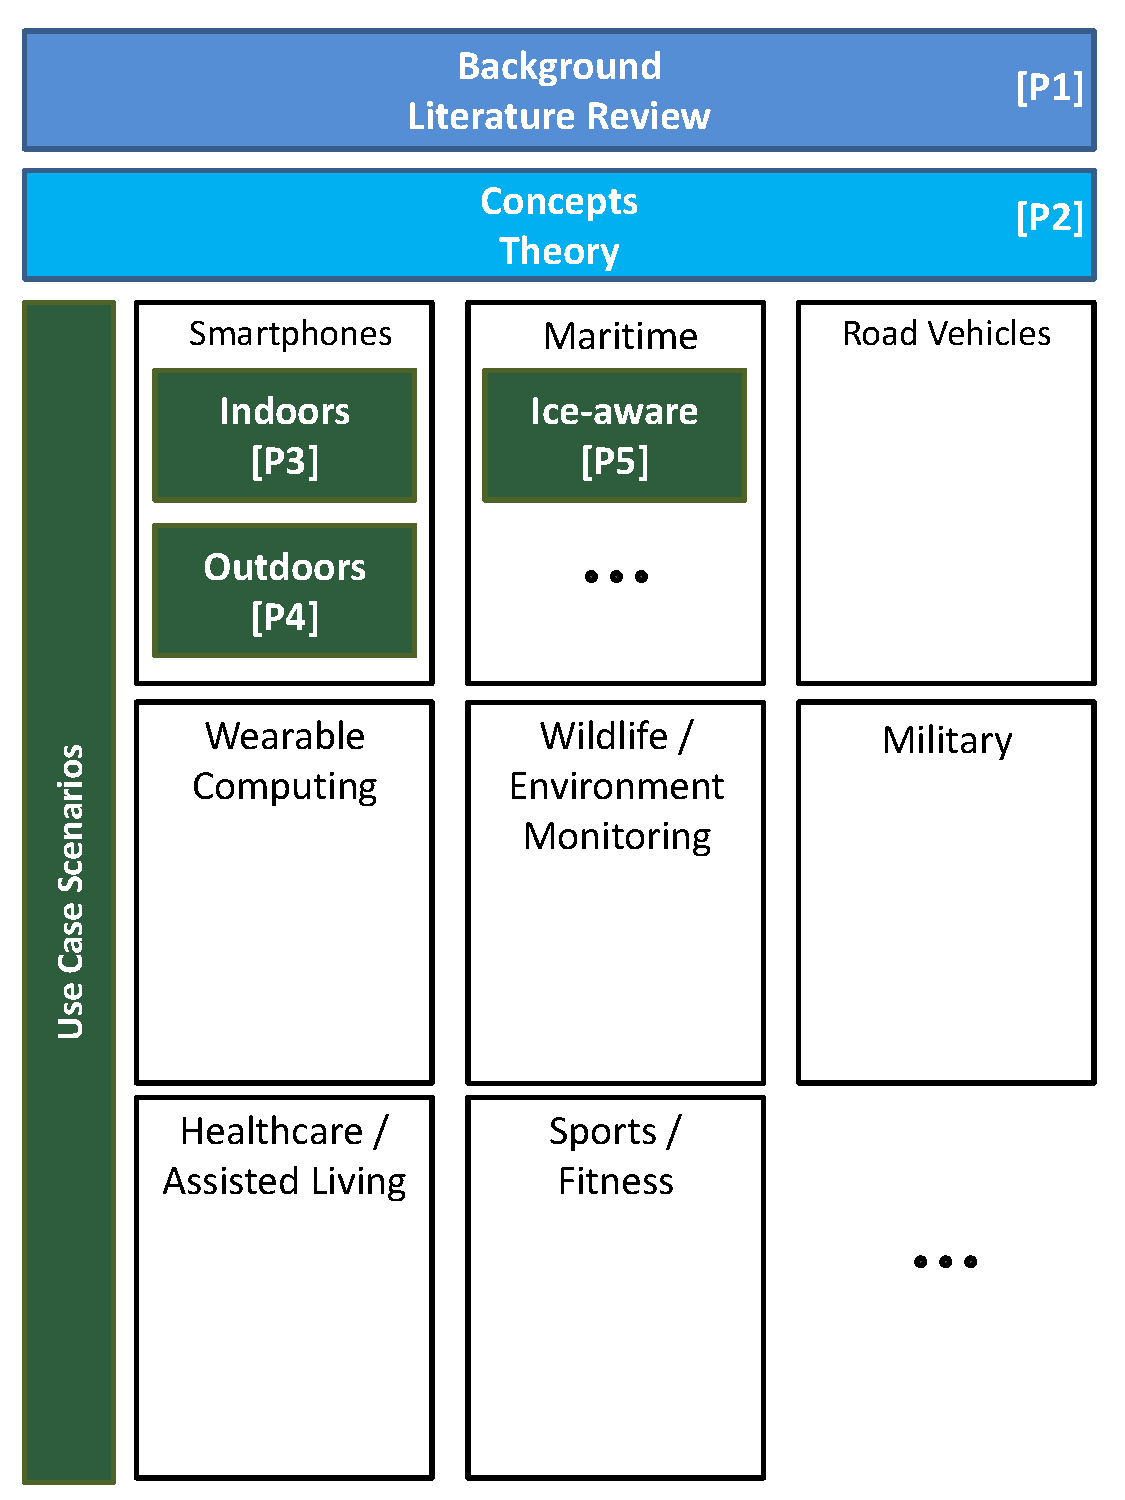
\includegraphics[width=1.0\textwidth]{Images/figChapter4}
  \end{center}
  \caption[Mapping of included publications to research areas]{Mapping of included publications to research areas. The additional empty boxes are intended to emphasize that many use case scenarios have yet to be explored. Further discussion on future use case scenarios can be found in Section~\ref{sec:future_applications}.}
  \label{fig:publication-chart}
\end{figure}

As Figure~\ref{fig:publication-chart} indicates, there are many potential use case scenarios that are not addressed in this thesis. There are, of course, many possible ways to categorize and sub-categorize the use cases, and this chart is not intended to be authoritative in this matter. The list is also not exhaustive. Our original research plan was to cover as many different use case scenarios as possible, but due to time constraints and project limitations, only two separate use case scenarios could be investigated (or three, if one considers [P3] and [P4] to cover separate use case scenarios). Our plans to cover additional use case scenarios will be discussed briefly in Chapter~\ref{ch:conclusions}.


\section{Author's Contributions to the Publications}
\label{sec:author_contributions}

This section outlines the main contributions of the author of this thesis to the included publications.

\textbf{[P1]:} The thesis author was the main author of this chapter, whereas the book co-author provided only editorial comments to a near-final draft. The thesis author conducted all the necessary background literature review and independently decided on the detailed contents of the chapter. The author also came up with the idea to use Hermagoras's ``seven elements of circumstance'' to organize and describe the different elements of context. The author also independently identified and collated the various Android \glsentrydescplural{api} (APIs) relevant to context awareness.

\textbf{[P2]:} The thesis author was the main author of this chapter, whereas the book co-author provided only editorial comments to a near-final draft. Similar to the case of [P1], the thesis author conducted all the necessary background literature review and independently decided on the detailed contents of the chapter. The author created all of the figures in the chapter and originated the concept of the ``context pyramid''. Finally, one of the main contributions of this chapter is the formulation and description (including figures) of rather complex mathematical concepts (e.g. \acrlong{svm}) in such a way that they are understandable to anyone with basic knowledge in algebra and probability.

\textbf{[P3]:} The thesis author was the second author of this publication, but the first author has affirmed in writing that the thesis author's contribution was roughly equal to that of the first author. The thesis author contributed equally to the design and implementation of the experiments. Implementation of the data collection application on a smartphone was primarily the responsibility of the thesis author. He also assisted in the analysis of the test results. In addition, he was the originator of the idea used for indoor-outdoor detection based on GPS signal-to-noise ratio and WiFi signal strength and implemented this method on a smartphone. The thesis author contributed to the development of the WiFi fingerprinting indoor positioning system and prepared the test environment by measuring and marking reference points and setting up additional WiFi access points. As stated earlier, he was the originator of the ``context pyramid'' concept, which is also described and employed in this paper. He was also the originator of the idea of using a graph-based grouping of the reference points. Lastly, he contributed to the preparation of the manuscript, including writing some sections and editing it in its entirety.

\textbf{[P4]:} The thesis author was the sole author of this publication and received assistance only in data collection, as well as general guidance from his supervisors. He also implemented all the necessary software used in the experiments, apart from the Weka software platform used in the data analysis. Some extensions to Weka, in terms of automating analysis and integrating Weka with Matlab, were also implemented by the author.

\textbf{[P5]:} The thesis author was the first author of this publication and was the originator of the idea of using a graph-based approach and the A* algorithm for ice-aware route optimization. He formulated the concept of combining a sea spatial model, ship maneuverability model, sea ice model, and ship performance model. In particular, the ship maneuverability model, which fixes the graph structure and discretizes the ship's maneuverability, was the thesis author's own invention. Furthermore, he implemented the optimization algorithm in Matlab, basing the implementation only roughly on an open source implementation.  The cost function was developed mainly by the thesis author, although various preliminary ideas were discussed together with the second author. The only parts of the method that were not implemented or provided by the thesis author were the resistive ship speed model, the ice data, and the historical ship data, all of which were provided by co-authors. Finally, the thesis author led the manuscript preparation, writing most sections, preparing all figures, and editing the manuscript in its entirety.
\chapter{Conclusions}
\label{ch:conclusions}

This chapter offers some conclusions based on this thesis, together with the included publications. It is organized as follows: Section~\ref{sec:summary} briefly summarizes the thesis. Section~\ref{sec:main_findings} outlines our main findings. Section~\ref{sec:future_work} describes our future work planned in the areas addressed by this thesis. Finally, Section~\ref{sec:concluding_remarks} provides a few concluding remarks.

\section{Summary}
\label{sec:summary}

The overall goal of this thesis was `to improve our understanding of how computing devices can better understand us and our needs. As argued in this thesis, such understanding if often embodied, at least partly, in a concept known as context awareness. The primary method used to endow computers with context awareness has been---and we argue it will continue to be---machine learning. 

In examining these topics, we have narrowed the focus to application areas related to navigation. Despite this narrowing of application areas, there are still many diverse needs in navigation, and this thesis focused on three particular use cases within navigation where context awareness is deemed beneficial: (1) detecting of different human activities inside a typical office environment to improve indoor location tracking, (2) detecting different ``mobility contexts'' of a smartphone user to improve outdoor location tracking, and (3) enabling ``ice aware'' route optimization for ships sailing in ice-covered waters to improve and automate the route planning needs of such ships. These use cases demonstrate the breadth of potential application areas of context aware technology. Three of the included publications ([P3]--[P5]) aim to improve the state-of-the-art in these application areas by introducing either novel methods, novel combinations of existing methods, or in-depth analysis of the performance of existing methods.

In addition to examining these application areas, this thesis has extensively reviewed the literature concerning context awareness and machine learning. In presenting and summarizing these topics, we have attempted to provide clear, tutorial-like examples, in order to aid readers unfamiliar with these subjects.

We have reviewed the early theoretical work in ``context'', led by artificial intelligence pioneer John McCarthy and others, while pointing out that generalizations of context have not led to significant breakthroughs in context-aware systems. In presenting the conceptual underpinnings of context awareness, we have introduced two conceptual frameworks for understanding context awareness and contextual reasoning. The first was adapted from the writings of an ancient Greek orator seven Hermagoras, known as the ``seven circumstances''. The second, which we have dubbed the ``context pyramid'' presents a division of the various steps in contextual reasoning into six levels ranging from raw data to ``rich context''. These two frameworks, general in nature, can assist the researcher and developer aiming to build context-aware systems by dividing the problem up into different categories of contextual information and steps in contextual processing.

On the topic of machine learning, this thesis has traced the history of the subject from its early beginnings with Arthur Samuel up to the modern notion. We have presented two major types of machine learning, supervised and unsupervised, using a toy problem, computer chess, as an example. We have emphasized the importance and benefits of automatic learning, despite the fact that supervised learning usually requires manual labeling of training data. Unsupervised learning, on the other hand, can largely meet the desire for automated learning, although it often requires some human interpretation of the results. The included publications provide further details on machine learning, and in particular [P3] and [P4] demonstrate the use of machine learning. The methods used in [P5] can be nominally considered machine learning, although most machine learning literature does not include search algorithms under this umbrella.

\section{Main Findings}
\label{sec:main_findings}

Below summarizes our main research findings:
%
\begin{itemize}
\item Context awareness is a broad and challenging topic, but one can find many beneficial applications of context awareness in the field of navigation.
\item Machine learning constitutes a powerful set of methods for endowing computers with context awareness.
\item A systematic evaluation of different available machine learning algorithms should be undertaken when applying machine learning to the problem of context awareness, especially if the aim is to maximize performance. The important fact is often overlooked by navigation researchers working on context awareness.
\item Context-aware smartphone applications are a present reality. Limited experiments have shown that a smartphone application could detect, e.g. various activities in an office setting and different outdoor mobility contexts, with high accuracy (\textgreater90\% for the former; \textgreater97\% for the latter).
\item As an example of a maritime application, awareness about ice conditions (as a function of space and time) can be exploited to perform automated route optimization. Such capability could augment or even replace the currently human-intensive task of route planning performed by crews of ships sailing in ice covered waters.
\item Many other applications of context awareness are evident in emerging technologies, and context awareness will play an even stronger role in the future, especially in so-called ``smart devices''.

\end{itemize}

\section{Future Work}
\label{sec:future_work}

In many ways, this thesis has only scratched the surface in exploring context awareness for navigation applications. In tackling the broader goal ``to improve our understanding of how computing devices can better understand us and our needs,'' we feel even less compelled to declare our work complete. This section outlines some of the planned future work in developing context-aware navigation applications.

Our future work can be divided into three broad categories: (1) future work in the three application areas covered by the included publications, (2) future work in new application areas, and (3) future work that can benefit context awareness broadly. The first category of future work will not be discussed further in this section because it is described in the included publications [P3]-[P5]. The other two categories will be discussed in separate sub-sections below.

\subsection{Future Applications}
\label{sec:future_applications}

In Figure~\ref{fig:publication-chart} we hinted at future application areas or ``use case scenarios''. Several of the highlighted use case scenarios are part of near future work. For example, in one recently initiated project, we aim to develop a ``tactical situation awareness system'' for soldiers.

Military applications of context awareness are particularly promising because the cost limitations are not as strict as in other application areas and specially-designed sensors can be installed, e.g. attached to various body parts of a soldier (helmet, boots, chest, etc.) or to other military equipment, providing a rich set of raw sensor data from which to generate context awareness. On the other hand, in military applications, reliability requirements are very high and typically there is a strong requirement for real-time functionality. For example, if a system is designed to detect when a soldier is in danger or injured, then false negatives, as well as false positives could prove very costly.

Another application area that has strong potential is healthcare and fitness monitoring. With the growing popularity of ``wearable devices,'' such as smartwatches and small heart-rate monitors, such applications have greater widespread consumer appeal. Many devices already exist that can, e.g. monitor calorie usage by tracking steps, but it remains a challenge to reliably and automatically detect different activities such as walking, running, cycling, hiking, etc. This is, of course, strongly overlapping with the topic of [P4], but we believe healthcare and fitness monitoring can go much beyond mere ``mobility context'' and incorporate other aspects, such as recognizing social interactions, detecting abnormal health or changes to a person's routine that might affect health and fitness, and warning users of dangerous or unhealthy situations. The concept of a ``personal health assistant'' is not really a matter of science-fiction but could be realized in the coming years. Context awareness and machine learning are the technologies that are likely to make this concept a reality.

\subsection{General Issues and Potential Solutions}
\label{sec:general_issues}

Lastly, we have noticed in our research several general issues that are relevant to context awareness in a broad sense. These issues are summarized as follows:
%
\begin{enumerate}
 \item Supervised learning requires labeled data, and labeled data is expensive.
 \item There is a lack of standardization in context awareness research.
 \item Many context awareness experiments are not easy to repeat or independently verify.
\end{enumerate}


The first general issue above is related to the use of supervised learning, which is often the adopted approach in many research works (such as in [P3] and [P4]). As mentioned in Section~\ref{sec:supervised-learning}, it can be very costly and time-consuming to generate the labeled data required to perform supervised learning. Furthermore, it is generally the case that the more data that can be collected, the more performant and reliable the resulting model will be. For example, if we are aiming to develop a context-aware smartphone application that works well across a large population of users, then we will need to collect training data from a large, diverse population of test users. This is very costly, especially in a research setting.

There are two potential solutions to this issue. The first is that researchers and developers would publish and share their training data. This would benefit the overall research community. We have practiced this approach in publication [P4], but generally this is not a common practice. The second approach would be to collect a sizable amount of labeled training data and then to supplement it with unlabeled data (which is less costly to collect). Performing machine learning using a combination of labeled and unlabeled data is known as \emph{semi-supervised learning}. This topic is outside the scope of this thesis but will be explored in our future work. As an example of this approach, a research and development team could collect a limited amount of labeled data using its own staff and volunteers and then supplement it with a large amount of crowdsourced unlabeled data. This is exactly the approach we are taking in a recently initiated project called MyGeoTrust (see \cite{Guinness2015}).

The second general issue has to do with standardization. To put it precisely, there is a lack of standardization in context awareness research, and this issue makes it difficult to compare results among different studies. As described in Chapter~\ref{ch:context_awareness}, context is understood in many different ways, and there is no one ``correct'' way to categorize and organize the context space.To provide an example, in publication [P4] we defined seven mobility contexts: walking, running, static, moving slowly, riding a train, riding bus, and driving. In a related study, four mobility contexts were defined: walking, running, bicycle, and land-based vehicle (including trains, metros, and cars) \cite{elhoushi2014robust}. A third study investigated another set of mobility contexts \cite{stenneth2013detecting}. The lack of standardization is so prevelent that there are nearly as many such definitions are there are studies of mobility context.

This lack of standardization is understandable, due to the fact that different researchers have different applications in mind and different ideas about how to segregate the context space, but it would be more beneficial for the overall research community if some level of standardization were applied. For example, one could propose one or more standard ontologies of context for various applications. Then, when presenting results researchers could reference these standards, i.e. ``the following classification results are according to standard X.Y...''. Also, there is no reason to limit results to one particular standard; data could be processed according to several different standards and presented in the same publication. We note that some work on contextual ontologies can be found in the literature, %TODO proide references
 but it is, in our view, an underdeveloped area. In our future work, we aim to contribute to and advance the notion of standard contextual ontologies.

The last general issue we would like to discuss is somewhat related to the second issue, and the solution is ironically similar to the first solution described above. One of the long-standing tenets of scientific research is reproducibility. Experiments should be described in enough detail so that other researchers can independently verify the results. In the case of context awareness research, this means that an independent researcher should be able repeat another researcher's data collection, apply the same algorithms, and achieve similar, if not identical, results. In reality, there are so many factors related to the environment, devices, and test subjects that collecting comparable data that produces comparable results is not realistic.

The solution is straight-forward. As an alternative, context researchers should publish the data upon which their results are based, along with sufficient documentation so that the data is usable by independent researchers. As already stated, this is rarely done in context awareness research. It is, however, a common practice in the machine learning community to test techniques against benchmark data. For example, the \gls{uci} maintains a repository of over 300 datasets that can be used for machine learning research. Unfortunately, very few of these datasets relate to context awareness. We aim to follow open data practices in our future work and also to actively promote this practice, either by promoting UCI's machine learning repository or by setting up a dedicated portal for context awareness research.

\section{Concluding Remarks}
\label{sec:concluding_remarks}

The remainder of this thesis consists of reprints of the five included publications described earlier. The order of the publications has been chosen to go from the most general to more specific and detailed applications. They can be read, however, in any order, depending on the reader's specific interests.



\setcounter{secnumdepth}{-1}
\chapter{Bibliography}
\bibliography{_rg_refs}%,Text/refs_3}
%\bibliographystyle{styles/IEEEtranS}
\bibliographystyle{ieeetr}
%%\input{references}

%\appendix
%\renewcommand{\chaptername}{Liite}

%\chapter{Liitteitä}

\end{document}

